\documentclass[10pt]{article}
\usepackage[utf8]{inputenc}
\usepackage[T1]{fontenc}
\usepackage{graphicx}
\usepackage[export]{adjustbox}
\graphicspath{ {./images/} }
\usepackage{amsmath}
\usepackage{amsfonts}
\usepackage{amssymb}
\usepackage{mhchem}
\usepackage{stmaryrd}
\usepackage{hyperref}
\hypersetup{colorlinks=true, linkcolor=blue, filecolor=magenta, urlcolor=cyan,}
\urlstyle{same}

\title{Drinking Water Operator Certification Training }

\author{}
\date{}


\begin{document}
\maketitle
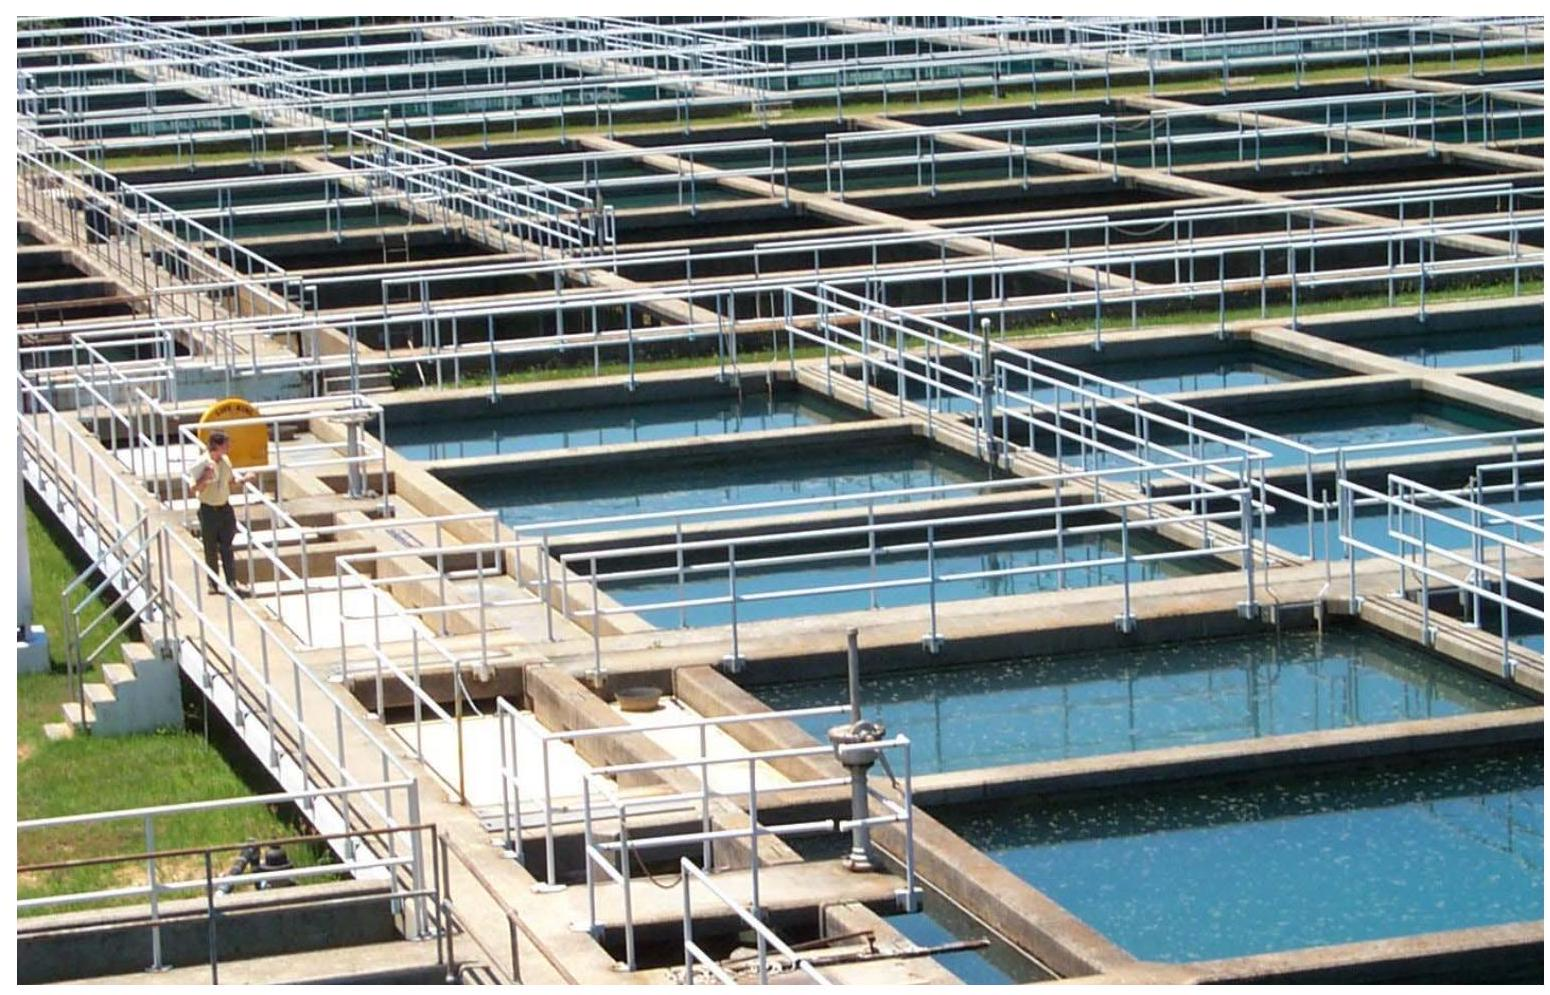
\includegraphics[max width=\textwidth]{2022_10_30_098bb5f44c5986ff92a9g-01}

\section{Student Manual}
\section{Module 8: Distribution Systems}
Revised July 2013

This course includes content developed by the Pennsylvania Department of Environmental Protection ( $\mathrm{Pa}$. DEP) in cooperation with the following contractors, subcontractors, or grantees:

The Pennsylvania State Association of Township Supervisors (PSATS)

Gannett Fleming, Inc.

Dering Consulting Group

Penn State Harrisburg Environmental Training Center

\section{Topical Outline}
\section{Unit 1 - Introduction to Operator Certification}
I. Certification\\
A. Certification Board\\
B. Operator Certification Act\\
C. Water Class E Certification

Unit 2 - Distribution Networks

II. Distribution Network Components\\
A. Introduction to Distribution Networks\\
B. Transmission Systems\\
C. Water Mains and Related Equipment\\
D. Distribution Storage\\
E. Distribution Pumping\\
F. Valves\\
G. Meters\\
H. Fire Hydrants\\
I. Backflow Prevention

III. Distribution Hydraulics\\
A. Pressure and Head\\
B. Energy Loss\\
A. Customers and Demands\\
B. Pressures and Flows\\
C. Routine Maintenance\\
D. Pipeline Maintenance

IV. System Performance

Unit 3 - Distribution Storage

I. Basic Principles\\
A. Purpose of Storage Facilities\\
B. Types of Storage Facilities II. Operations

$\| l$.\\
A. Storage Volume and Water Level\\
B. Operating Procedures\\
Maintenance\\
A. Purpose of Distribution Storage Maintenance\\
B. Painting\\
C. Corrosion Control\\
D. Water Quality

Unit 4 - Water Quality and Monitoring

I. Distribution Systems Water Quality Issues\\
A. Chemical\\
B. Biological\\
C. Aesthetic\\
Disinfection in Distribution Systems\\
A. Purpose of Disinfection\\
B. Disinfection Chemicals\\
C. Chlorine Residual\\
D. Disinfection of New Mains and Storage Facilities

III. Monitoring Distribution Systems Water Quality\\
A. System Classifications\\
B. Regulatory Monitoring and Sampling Locations\\
C. Operations Monitoring\\
D. Other Monitoring

IV. Practices To Enhance Water Quality\\
A. Distribution Flushing\\
B. Cross Connection Control\\
C. Water Main Cleaning and Lining\\
D. Minimization of Dead Ends and Residence Times\\
E. Chlorine Booster Facilities\\
F. Corrosion Control\\
G. Storage Facility Operations

\section{Unit 1 - Introduction to Operator Certification}
\section{Learning Objectives}
\begin{itemize}
  \item Introduce distribution operator certification regulations.

  \item Discuss operator certification continuing education requirements.

  \item Discuss intended results of certification regulations.

  \item Identify the use of process control decisions and standard operating procedures.

\end{itemize}
\section{Distribution Operator Certification Regulations}
Water and Wastewater Operator Certification Program Regulations, Chapter 302

\begin{itemize}
  \item The regulations are intended to protect the environment and ensure the public's health and safety. To accomplish this goal, the program only certifies individuals with the correct knowledge, skills, and abilities.

  \item Establishes standards for operator certification, recertification, certification renewal and security training; defines the certification renewal period and requirements for certification renewal.

  \item Requires certified operators for water distribution systems.

  \item To become certified in distribution systems, a person must successfully complete the "Water Class E - Distribution System" certification examination and meet work and educational experience qualifications. Once they have passed the examination, they may submit an application along with a criminal background check to the Certification Board.

\end{itemize}
The Operator Certification Board has the authority to approve or deny applications for new certifications, renewals, upgrades, downgrades, and license reciprocity.

Once certified, an operator is required to meet continuing education requirements to maintain their certification.

\begin{itemize}
  \item To maintain a distribution license, operators must complete 8 hours of continuing education in the first 3 year cycle and 15 hours of continuing education in each subsequent 3 year cycle.

  \item You are not able to bank continuing education hours and you are not able to carry over any remaining hours to the next cycle.

  \item Only continuing education approved by the Department of Environmental Protection will count.

  \item Duplicate training courses (same DEP course ID) taken in the same cycle will not count towards required continuing education credit.

\end{itemize}
$\square$ Failure to meet continuing education requirements within the three year period will result in the loss of certification.

\begin{itemize}
  \item There is no grace period.

  \item In the event the operator would decide to be certified again, they would be required to start the entire process over again. An available operator must make all process control decisions for the system.

  \item A process control decision is any decision that changes or maintains water quality or water quantity of a water system or wastewater system in a manner that may affect the public health or the environment.

  \item This means that any action which has an impact on the water quality or water quantity must be made by a certified operator or by another person following standard operating procedures written and approved by the certified operator for the system.

  \item Uncertified and not appropriately certified operators can only make process control decisions when under direction of an appropriately certified operator or using Standard Operating Procedures that were developed by an appropriately certified operator.

  \item An example would be if an operator wanted to divert more water flow in a system toward a tank, and as a result, they closed some valves to accomplish this objective. This action caused an increase in quantity of water in that particular section of main line and therefore is considered a process control decision.

\end{itemize}
$\square$ Additional Operator Responsibilities: In addition to making process control decisions, the certified operator is required to inform the owner/management of the system of any issues that may be or are causing violations of the regulations or permit conditions.

\begin{itemize}
  \item The system owner is responsible for taking appropriate actions in a timely manner to the reports of operators
\end{itemize}
\section{Key Points for Unit 1 - Operator Certification}
\begin{itemize}
  \item Water and Wastewater Operator Certification Program Regulations establishes standards for operator certification, recertification, certification renewal and security training; defines the certification renewal period and requirements for certification renewal.

  \item Failure to meet continuing education requirements within the three year period will result in the loss of certification.

  \item A process control decision is any decision that changes or maintains water quality or water quantity of a water system in a manner that may affect the public health or the environment. Process control decisions must be made by an appropriately certified operator.

\end{itemize}
\section{Unit 1 Exercise}
\begin{enumerate}
  \item To become certified in distribution systems, a person must:\\
a.\\
b.\\
C.

  \item Give an example of a process control decision that must be made by a certified operator or by another person following standard operating procedures written and approved by the certified operator for the system:

  \item Please determine whether a certified operator, system owner, or Certification Board is responsible for each of the following actions:

\end{enumerate}
\section{Action:}
Approve a new application for certification:

Report any situations causing a violation to the system owner:

A process control decision:

Respond to a certified operator report:

\section{Unit 2 - Distribution Networks}
\section{Learning Objectives}
\begin{itemize}
  \item Identify the key components of a distribution network and describe the primary purpose or function of each component.

  \item Define the relationship among pressure, head, and hydraulic grade line.

  \item Outline the relationship between distribution system customers' demands and their effects on distribution system performance.

  \item $\quad$ Relate how pressures and flows are used to gauge distribution system performance.

  \item List five programs involved in routine maintenance of distribution networks.

  \item List three key components of a pipeline maintenance program.

\end{itemize}
\section{Introduction to Distribution Networks}
\section{Purposes of Distribution Networks}
The primary purpose of a distribution network is to deliver adequate volumes of safe drinking water to system customers at adequate pressures.

Another important purpose of a distribution network is to provide adequate fire flows to areas of the system.

\section{Components of Distribution Networks}
Pipes

Storage Facilities

Pumps

Valves

Hydrants

Meters

\includegraphics[max width=\textwidth]{2022_10_30_098bb5f44c5986ff92a9g-11}

Figure $2.1$ - Distribution System Layout

\section{Purpose of Transmission Systems}
\section{Transmission Systems}
Transmission systems are used to convey water from a system's source of supply to the distribution network.

\section{Typical Characteristics of Transmission Systems}
Large diameter pipelines

May be miles in length

Typically, no service connections directly from a transmission system

\section{Water Mains and Related Equipment}
\section{Pipe Features}
Size

\begin{itemize}
  \item Distribution network pipes are normally sized to accommodate normal and peak system flows and fire flows without adversely impacting water quality or resulting in an excessive pressure drop.
\end{itemize}
\section{Material}
\begin{itemize}
  \item Distribution network pipes are constructed of material that is durable and corrosion resistant.

  \item Materials currently used for distribution network pipes include ductile iron, steel, concrete, and plastic.

  \item Materials often used for older pipes in a distribution network include cast iron, asbestos cement, galvanized iron, and wood.

\end{itemize}
\section{Pressure Rating}
\begin{itemize}
  \item The pressure rating of a pipe is a measure of the maximum normal pressure that a pipe is able to withstand.

  \item The pressure rating of a pipe will vary based on pipe material and pipe class. Joints

  \item Connect two pipe segments.

  \item Types of joints include: push-on, mechanical, flanged, mechanical couplings, sleeve, welded, and harness or restrained sleeves.

  \item The type of joint used is dependent upon the pipe material and installation conditions. Pipe joints for buried pipes need to provide some flexibility.

\end{itemize}
\includegraphics[max width=\textwidth]{2022_10_30_098bb5f44c5986ff92a9g-13}

Figure $2.2$ - Push-on Joint ${ }^{1}$

\includegraphics[max width=\textwidth]{2022_10_30_098bb5f44c5986ff92a9g-13(1)}

Figure $2.4$ - Flanged Joint 3

\includegraphics[max width=\textwidth]{2022_10_30_098bb5f44c5986ff92a9g-13(2)}

Figure $2.3$ - Mechanical Joint ${ }^{2}$

\includegraphics[max width=\textwidth]{2022_10_30_098bb5f44c5986ff92a9g-13(3)}

Figure $2.5$ - Mechanical Coupling Joint 4

\section{Fittings}
\begin{itemize}
  \item Fittings can be used to connect pipes of the same or different size, change the direction of flow, or stop flow.

  \item Typical fittings include sleeves, reducers, bends, tees, and caps.

\end{itemize}
\section{Basic Water Main Installation}
Water main installation begins with excavation. Excavation for water main installation is expensive and dangerous.

Preparations for excavation must be made in advance so the job will run smoothly, efficiently, and safely. The Occupational Safety and Health Administration has information and training that is recommended. OSHA documents that each month, 2 workers are killed when a trench collapses. Get educated on trench safety before ever entering a trench. Trench steps include:

\begin{enumerate}
  \item Before excavation can begin, the project must be well planned and safety must be a consideration.

  \item To protect the trench and workers from traffic, the excavated material should be piled on the pavement side of the trench.

\end{enumerate}
\begin{itemize}
  \item Place all excavated or fill materials a minimum of two feet away from the top edge of the trench. If materials need to be closer than two feet from the edge of the trench, install an effective barrier to prevent them from falling into the excavation.
\end{itemize}
\begin{enumerate}
  \setcounter{enumi}{3}
  \item Before entering the trench, determine if shoring is necessary.
\end{enumerate}
\begin{itemize}
  \item OSHA requires a protective system for trenches 5 feet or greater.
\end{itemize}
\begin{enumerate}
  \setcounter{enumi}{4}
  \item Determine if a hazardous atmosphere exist in the trench.
\end{enumerate}
\begin{itemize}
  \item $\quad$ Normal oxygen levels range from $19.5$ to $21.5 \%$.
\end{itemize}
\begin{enumerate}
  \setcounter{enumi}{5}
  \item Determine if access to and exit from the trench is required.
\end{enumerate}
\begin{itemize}
  \item Trenches 4 feet or more in depth must have a safe means of egress.

  \item Spacing between ladders or other means of egress must be such that a worker will not have to travel more than 25 feet laterally to the nearest means of egress.

  \item Ladders must be secured and extend a minimum of 36 inches above the landing.

\end{itemize}
After the trench is prepared, inspect the pipe.

\begin{itemize}
  \item Inspect the pipe for defects, damage, oil, dirt, grease, and/or foreign matter.

  \item Any unsound material should be replaced and all foreign matter or dirt should be removed from the interior of the pipe before lowering into the trench.

\end{itemize}
Before lowering the pipe into the trench the trench bottom should be smooth and free of material like large stones or large dirt clods.

Lower the pipes, and other necessary equipment carefully into the trench.

Before connecting the pipe:

\begin{itemize}
  \item Inspect the bell to be sure that no dirt or foreign material is on the ring.

  \item Clean the pipe end around the entire circumference from the end spigot to 1 inch above the reference line (note: this line is used for proper insertion depth of bell and spigot).

  \item Once the pipe is cleaned, be careful during installation to ensure gravel does not enter into the line.

\end{itemize}
Be sure to use blocks or restraints to avoid leaks and pipe movement from the thrust against tees, valves, bends, reducers and fire hydrants.

\begin{itemize}
  \item Size and type of the thrust block depends on maximum pressure, pipe size, kinds of soil and types of fittings. After the water main pipe and fittings have been installed in the trench, the excavation must be backfilled with suitable material.

  \item Only clean sand or selected soil should be used for the first layer. The bedding around the pipe should be of uniform size and material. Allowing materials of various sizes such as large rocks could cause the pipe to fracture during settlement.

  \item The first layer of backfill should be placed equally on both sides of the pipe, up to about the center of the pipe. This material should then be compacted, a process often called haunching.

  \item Depending on the area and conditions, generally another layer of backfill is placed over the pipe and again compacted to protect and secure the pipe.

  \item The trench needs refilled appropriately. The backfill material should be compacted at 12 inch intervals to minimize settlement.

  \item Backfill practices vary depending on type of pipe, local soil conditions and regulatory requirements. Proper backfilling is very important:

  \item Improper compaction = broken lines

  \item Large backfill = increase probability of main break

\end{itemize}
All new sections of water mains must be thoroughly disinfected.

\begin{itemize}
  \item To properly disinfect water mains, different methods can be applied. Due to the dangers of chlorine it is advised that the operator choose the best method that suits the facility's needs.

  \item Calcium hypochlorite tables can be placed in each section of pipe and fire hydrant as work progresses.

  \item A concentrated chlorine solution can be injected through a corporation stop.

  \item The chlorination rate should be such that it will produce a concentration of about $50 \mathrm{mg} / \mathrm{L}$ when mixed with incoming water.

  \item Mathematical calculations are necessary to determine how much chlorine will be needed.

  \item This will be addressed in the chlorination section.

  \item The chlorine solution should remain in the pipe for at least 24 hours.

\end{itemize}
After the trench has been backfilled, the new main must be pressure tested to determine whether there are any leaks.

\begin{itemize}
  \item The test may be performed one section at a time between valves or the installer may wait and test the entire job at one time.
\end{itemize}
At the end of the contact period, the chlorinated water should be flushed from the pipeline.

\begin{itemize}
  \item One or more fire hydrants should be used for flushing so that a velocity of around $5 \mathrm{ft} / \mathrm{s}$ is obtained in the pipe.

  \item This velocity should be maintained long enough to allow two or three complete changes of water and for the water to run visibly clean. - Gravel in the line is an indication of improper installation.

  \item The highly chlorinated water will probably kill grass, so the flow should be carried to a disposal site through hoses.

  \item In some cases, the water may need dechlorinated before it is released to a waterway.

\end{itemize}
After a new pipeline has been disinfected and flushed, it should be refilled with water from the distribution system and tested for bacteriological quality.

\begin{itemize}
  \item This test takes at least 24 hours to complete from the time of sampling.

  \item The test must meet requirements of the Department of Environmental Protection.

\end{itemize}
\section{Service Connections}
\includegraphics[max width=\textwidth]{2022_10_30_098bb5f44c5986ff92a9g-17}

Figure $2.6$ - Typical Customer Service Connection

Service lines are used to convey water from the distribution network to individual system customers. Typical materials used for service lines include plastic, copper, steel, iron and lead. Lead service lines are being neutralized by corrosion control practices or are being removed from service.

A corporation stop or shut-off valve is typically located at the connection of the service line and distribution pipe. Typically tapped at 10:00 o'clock or 2:00 o'clock positions.

An additional shut-off valve, the curb stop, is typically located along the service line, near the customer property line.

\includegraphics[max width=\textwidth]{2022_10_30_098bb5f44c5986ff92a9g-17(1)}

Figure $2.7$ - Typical Curb Stop

The customer meter used for billing purposes is located on the downstream side of the curb unit stop.

Backflow prevention devices are installed at customer meters or between the meter and the customer's line to prevent contamination of the distribution network from potential backflow.

\section{Distribution Storage}
\section{Storage Facilities}
Storage tanks are a common component in most water distribution systems.

$\square$ Help offset fluctuations in system demands;

Help minimize fluctuations in system pressure;

Elevated tanks are used to provide pressure in distribution systems

Provide reserve volumes of water to help meet fire flow needs; and,

Provide an emergency source of supply for the system.

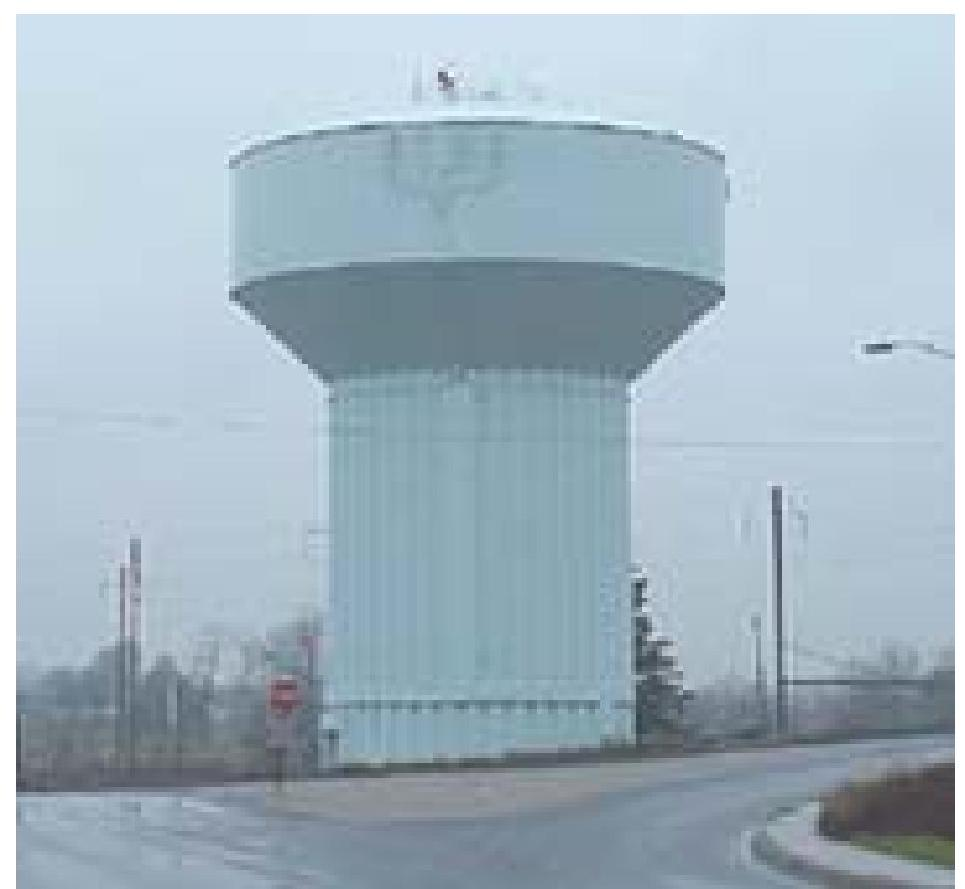
\includegraphics[max width=\textwidth]{2022_10_30_098bb5f44c5986ff92a9g-18}

Figure $2.8$ - Typical Water Storage Tank in the Distribution System

\section{Purpose of Pumps}
\section{Distribution Pumping}
The purpose of a distribution pump is to provide the energy necessary to lift water from lower elevations to higher elevations.

\section{Pump Terms and Definitions}
Flow-the volume of water per unit of time that passes through a pump. Typical units of measure for flow include gallons per minute (gpm), cubic feet per second (cfs), and gallons per day (gpd).

Pump Head-the amount of energy input to the water by the pump. Pump head is typically measured in units of feet of water (ft).

Water Horsepower-the amount of power supplied to the water which is needed to pump water to a certain elevation. Water Horsepower is typically measured in units of horsepower (hp).

Brake Horsepower-the amount of power that must be applied to the pump shaft to operate the pump. This is higher than the water horsepower since there are inefficiencies in the pump and motor, where energy is lost to friction and heat. Brake Horsepower is typically measured in units of horsepower (hp).

Pump Efficiency-the percentage of the power input to the shaft, that is actually transferred to the water.

\section{Example $2.1$ - Water Horsepower Calculation}
A centrifugal pump with an efficiency rating of $80 \%$ is used to pump water in a distribution system. If the brake horsepower applied to the centrifugal pump is 4 horsepower (hp), how much water horsepower is conveyed to the water by this centrifugal pump?

Efficiency e $=0.80=$ power output $/$ power input $=$ water horsepower $/$ brake horsepower

This equation can be rearranged to give water horsepower $=(0.80) \mathrm{x}$ brake horsepower, or: water horsepower $=(0.80) \times(4$ horsepower $)=3.2$ horsepower.

\section{Valves}
\section{Purpose of Valves}
The primary purpose of valves is to allow for isolation of mains or sections of main within the network.

Another important function of valves is to control flow or pressure.

\section{Valve Applications}
Isolation Valves are used to isolate mains or sections of mains.

\begin{itemize}
  \item Isolation may be necessary when repairing main breaks or leaks or performing other distribution network maintenance activities.

  \item The most commonly used isolation valve is the gate valve. Gate valves should NOT be used to throttle flow.

\end{itemize}
\includegraphics[max width=\textwidth]{2022_10_30_098bb5f44c5986ff92a9g-20}

Figure $2.9$ Gate Valve ${ }^{5}$

Control Valves are used to control flow or pressure in an area of the distribution network.

\begin{itemize}
  \item Flow control valves can be used to throttle or limit flow, change flow direction, and prevent reverse flow (check valves and backflow prevention valves). An example of a flow control valve is a butterfly valve. It typically has several set positions and can be adjusted to allow various flows through piping.

  \item Altitude valves are types of flow control valves that control flow in and out of storage facilities based on water level. When a tank reaches a maximum level the valve closes, preventing the tank from overflowing. When the water level in the tank drops due to system demands, the valve opens. - Pressure control valves can be used to reduce pressure (pressure reducing valves), maintain pressure (pressure sustaining valves), and protect against overpressure (pressure relief valves). Pressure reducing valves are used to create headloss and "break" pressure to keep system pressures less than the pressure ratings in pipes and to avoid other adverse impacts of high pressure.

\end{itemize}
\includegraphics[max width=\textwidth]{2022_10_30_098bb5f44c5986ff92a9g-21}

Figure $2.10$ - Pressure Reducing Valve ${ }^{6}$

Air Release Valves are used to eliminate air from a distribution network or to allow air into a distribution network.

\begin{itemize}
  \item Air relief or air release valves relieve pockets of air which typically accumulate at high elevation points in a distribution network.

  \item Vacuum relief valves allow air into the distribution network to protect the system against low pressures, including vacuum conditions. Vacuum relief valves are commonly used along transmission mains and at the discharge of pump stations to protect against low pressures that can occur as a result of sudden large changes in flow velocity.

\end{itemize}
\includegraphics[max width=\textwidth]{2022_10_30_098bb5f44c5986ff92a9g-21(1)}

Figure $2.11$ - Air Release Valve ${ }^{7}$

Isolation valves should be located in a manner that will limit service interruptions during emergency repairs and general maintenance.

\begin{itemize}
  \item General rule of thumb regarding location of isolation valves: isolating a segment of main should require operation of no more than 4 valves.
\end{itemize}
Check valves are used in distribution systems to prevent backflow. Check valves allow flow in only one direction.

\section{Valve Operation}
Valves can be operated manually or automatically via control systems.

When operating a valve manually, the approximate number of turns required to fully open or close a valve can be calculated as follows:
$$
\text { \# of turns = (Diameter of the valve (in inches) } \times 3)+3
$$
Table 2-1

\begin{tabular}{|c|c|}
\hline
Valve Size & Number of Turns \\
\hline
4 inch & $14 \frac{1}{2}$ \\
8 inch & 27 \\
12 inch & $38 \frac{1}{2}$ \\
16 inch & 53 \\
\hline
\end{tabular}

\section{Sample Calculation}
Approximately how many turns would it require to fully close a typical 6-inch valve that is initially fully opened?

Ans: $\#$ of turns $=(6 \times 3)+3=21$ turns

The direction (clockwise or counter clockwise) used to open or close a valve can vary from valve to valve. The proper direction to open the valve is usually indicated by an arrow on the valve bonnet. However, most systems typically standardize all valves in the system to operate the same.

When exercising a valve, the operator should make sure that a valve is properly returned to its original position. This is done by considering the number of valve turns required to fully open or close the valve.

When exercising valves, be aware of water hammer.

\begin{itemize}
  \item Water hammer is the momentary increase in pressure inside a pipe caused by a sudden change of direction or velocity of the liquid in the pipe. Basically, water rushing through a pipe comes to an abrupt stop. The sudden stop creates a shock wave.

  \item Water hammer can cause pressure spikes 10 times higher than normal operating pressures.

  \item Water hammer can be particularly dangerous because the increase in pressure can be severe enough to rupture a pipe or cause damage to equipment.

  \item Therefore, to avoid water hammer, slowly open and close valves.

\end{itemize}
\section{Meters}
\section{Purpose of Meters}
Meters measure, display, and record the amount of water that passes through a distribution system component.

\section{Meter Uses}
Typical applications of meters in a distribution network include:

$\square \quad$ Measuring the amount of water supplied to the system.

Measuring the amount of water supplied to a particular area of the system, including through a pump station or control valve.

Measuring the amount of water used by a customer, for billing purposes.

Monitoring unaccounted-for water in a distribution network.

\section{Types of Meters}
\section{Displacement Meters}
\begin{itemize}
  \item Commonly used as customer service meters.

  \item Typically have diameters of 2-inches or less.

  \item Generally used to measure low flow rates.

  \item Have limitations at very high flows.

\end{itemize}
\includegraphics[max width=\textwidth]{2022_10_30_098bb5f44c5986ff92a9g-23}

Figure $2.12$ - Displacement Meter ${ }^{8}$

\section{Velocity Meters}
\begin{itemize}
  \item Commonly used in pump stations, industrial facilities, and large diameter mains to measure high rates of flow.

  \item Do not accurately measure low flow rates.

  \item Include the Venturi, Turbine, and Propeller type meters.

\end{itemize}
\includegraphics[max width=\textwidth]{2022_10_30_098bb5f44c5986ff92a9g-23(1)}

Figure $2.13$ - Velocity Meter ${ }^{9}$

\section{Compound Meters}
\begin{itemize}
  \item Commonly used to measure flow at apartment complexes, schools, and industries that can typically have high peaks in water use compared with daily averages.

  \item Composite of the displacement and velocity meters.

  \item Used to measure flowrates that vary widely.

\end{itemize}
\includegraphics[max width=\textwidth]{2022_10_30_098bb5f44c5986ff92a9g-24}

Figure $2.14$ - Compound Meter ${ }^{10}$

\section{Electric Meters}
\begin{itemize}
  \item Measure flow magnetically (mag meter) or sonically.

  \item Highly accurate if properly located.

\end{itemize}
\includegraphics[max width=\textwidth]{2022_10_30_098bb5f44c5986ff92a9g-24(1)}

Figure $2.15$ - Electronic Meter ${ }^{11}$

\section{Proportional Meters}
\begin{itemize}
  \item Measure high flowrates at locations such as fire service lines.

  \item Do not measure low flows accurately.

\end{itemize}
\includegraphics[max width=\textwidth]{2022_10_30_098bb5f44c5986ff92a9g-24(2)}

Figure $2.16$ - Proportional Meter ${ }^{12}$

\section{Fire Hydrants}
\section{Purpose of Fire Hydrants}
The primary purpose of a fire hydrant is to provide water at high flow rates to aid in extinguishing fires.

Fire hydrants can also be used for flushing pipelines in the event of taste and/or odor complaints.

Fire hydrants can be used for supplying water to water trucks and construction equipment.

\section{Types of Fire Hydrants}
Dry-barrel hydrants

Include a shut-off valve and drain. The drain is open when the hydrants main valve is fully closed (otherwise the water left in the barrel once the main valve closes cannot escape and might freeze).

Wet-barrel hydrants

Will always be charged (have water in the hydrant). Have a shutoff valve at the outlet and can only be used in areas where freezing is not a concern.

\includegraphics[max width=\textwidth]{2022_10_30_098bb5f44c5986ff92a9g-25}

Figure $2.17$ - Dry Barrel Hydrant ${ }^{13}$

\section{Nozzles}
Hydrants generally have three nozzles

\begin{itemize}
  \item Two $2 \frac{1}{2}$-inch nozzles, and

  \item One $4 \frac{1}{2}$-inch nozzle (pumper connection).

\end{itemize}
$\square$ Protective caps for the nozzle heads are necessary to safeguard the nozzle threads.

\section{Fire Hydrant Coding}
Fire companies need to be able to quickly determine which tactics they should employ and how best to supply themselves with water.

\begin{itemize}
  \item They need to know how much water is available from the closest hydrant.

  \item The water pressure in each hydrant.

\end{itemize}
The most efficient means to convey this important information is to paint the hydrant tops and caps using standardized color codes. See table 2-2 for NFPA color coding. Table 2-2

\begin{tabular}{|c|c|c|}
\hline
\multicolumn{3}{|c|}{NFPA Top Colors} \\
\hline
Color & GPM & Rating \\
\hline
Blue & 1500 or more & Very good flows \\
\hline
Green & $1000-1499$ & Good flow for residential \\
\hline
Orange & $500-999$ & Marginally adequate flow \\
\hline
Red & Below 500 & Inadequate flow \\
\hline
\end{tabular}

\section{Locations of Fire Hydrants}
Hydrants should be easily accessible.

The maximum distance between hydrants in a distribution network ranges from 300 to 600 feet, depending on the area served.

\section{Basic Fire Hydrant Installation}
Before installing a new hydrant, test the hydrant by opening and closing to ensure no damage occurred during storage or shipping.

Also, before installing a hydrant, ensure that the hydrant meets local standards.

\begin{itemize}
  \item Most hydrants open counterclockwise and have operating nuts that measure $1 \frac{1}{4}$ in.
\end{itemize}
Depth of burial should be carefully computed and checked to make sure the hydrant to be installed will stand the correct distance above the ground.

\begin{itemize}
  \item The breakflange should be located about 2 inches above the ground surface.
\end{itemize}
Hydrants are typically located at street intersections so a hose can be strung in any direction for flushing.

\begin{itemize}
  \item Hydrants should be located far enough back from a roadway to minimize the danger of being struck by vehicles.
\end{itemize}
When installing a hydrant, a hydrant must be set on firm footing that will not rot or settle.

\begin{itemize}
  \item A flat stone or concrete slab is ideal.

  \item Hydrants must also be securely blocked or restrained from movement because the force against it will be tremendous if the valve is closed too quickly.

  \item To facilitate quick removal of the water from the hydrant barrel when the main valve is shut, a pocket of coarse gravel or crushed rock should be placed in the excavation before the hydrant is set.

  \item The gravel or stone should start at the bottom of the trench and continue to at least 6 inches above the hydrant drain.

\end{itemize}
\section{Fire Hydrant Operation Tips}
Always stand on the side of the hydrant without a cap when opening to prevent injury from the caps or barrel, which are under pressure and may become dislodged.

Count the number of turns when operating a hydrant to ensure full opening or closing of the shutoff valve.

Open and close the hydrant shut-off valve slowly to minimize potential pressure surges in the system.

When possible, open the hydrant shut-off valve fully when operating to prevent excessive wear that can be caused by partially opening the valve. If the flow from a hydrant needs to be regulated, it can be accomplished through a portable valve which is attached to the hydrant nozzles.

Hydrants should be exercised at least once per year. When exercising hydrants, hydrant maintenance should include operating valve, inspecting and greasing threads using a food grade lubricant, and insuring drainage in dry barrel hydrants.

\section{Backflow Prevention}
Backflow-is the flow of water, or mixture of water and other substances, from a source other than an intended source into the distribution network. Backflow can occur when the pressure at the unintended source, often a customer connection, is greater than the pressure in the distribution network.

\section{Purpose of Backflow Prevention}
To prevent potential contaminants from being introduced to the distribution network by the reverse flow of water from a source of questionable water quality.

\section{Types of Backflow Prevention Devices}
A physical air gap or separation between the backflow source and the distribution network.

A reduced pressure device (double-check valve with relief valve as added redundancy).

Vacuum Breaker

A double-check valve assembly.

\section{Pressure and Head}
\section{Terms and Definitions}
Pressure - the force per unit of area. Pressure is commonly expressed in units of pounds per square inch (psi).

Pressure Head - the vertical distance from a free water surface to a point below the surface (i.e., pressure increases with increasing depth). Pressure head is commonly expressed in units of feet of water (ft). This is because the only factor influencing pressure in a column of water is the elevation of the water in question. The volume of water does not matter as the pressure is measured in pound per square inch increments at the base of the unit.

\section{Relation between Head and Pressure}
Pressure, psi = Pressure Head, ft / 2.31, or

Pressure, psi x $2.31=$ Pressure Head, ft

Water pressure is directly related to the height (depth) and density of water.

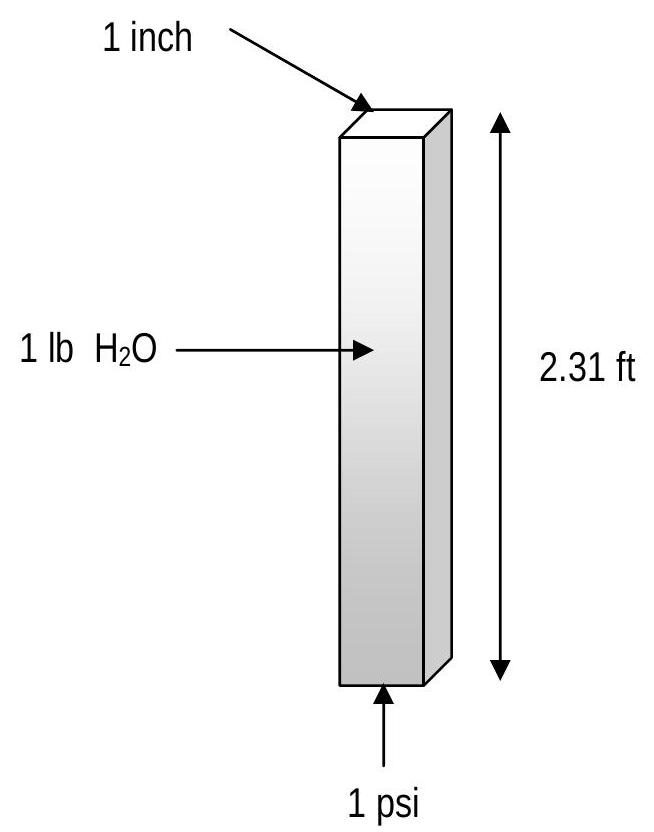
\includegraphics[max width=\textwidth]{2022_10_30_098bb5f44c5986ff92a9g-28}

$\underline{1 \mathrm{lb}}=2.31 \mathrm{ft}$ or $1 \mathrm{psi}=2.31 \mathrm{ft}$ inch $^{2}$

Pressure is described in units of pounds per square inch. For every $2.31 \mathrm{ft}$ of water, $1 \mathrm{lb}$ of pressure is exerted on one square inch.

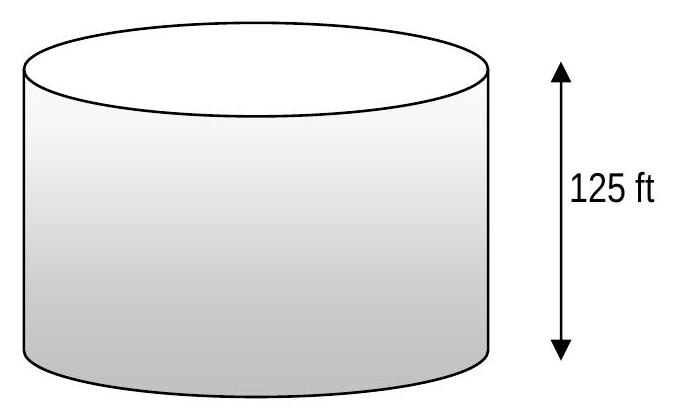
\includegraphics[max width=\textwidth]{2022_10_30_098bb5f44c5986ff92a9g-29}

How much pressure does water exert on both tanks if they are filled to the top (psi)?

Note: pressure is not affected by the volume of the tank, only the height. Both tanks are the same height; therefore both tanks will exert the same amount of pressure on 1 square inch.
$$
\text { psi }=\frac{1 \mathrm{psi}}{2.31 \mathrm{ft}} \times \underline{125 \mathrm{ft}}=\frac{125 \mathrm{psi}}{2.31 \mathrm{ft}}=54.1 \mathrm{psi}
$$

\section{Example 2.2 - Pressure Head Calculation}
How many feet of water would be in a tank if the pressure gauge at the base of the tank read 15 psi?

\section{Example 2.3 - Pressure Head Calculation}
What would the pressure head in psi be on a fire hydrant if a pressure gauge on that fire hydrant read 258 feet?

\section{Example $2.4$ - Pressure Head Calculation}
What is the pressure (in psi) at a point 12 feet below the surface? Hydraulic Grade Line (HGL) - the height to which a column of water will rise if you placed a vertical riser pipe on a pipe under pressure.

The HGL in a pressure pipe is the imaginary water level at that point along the pipeline, if the pressure or head was not restrained within the pipe.

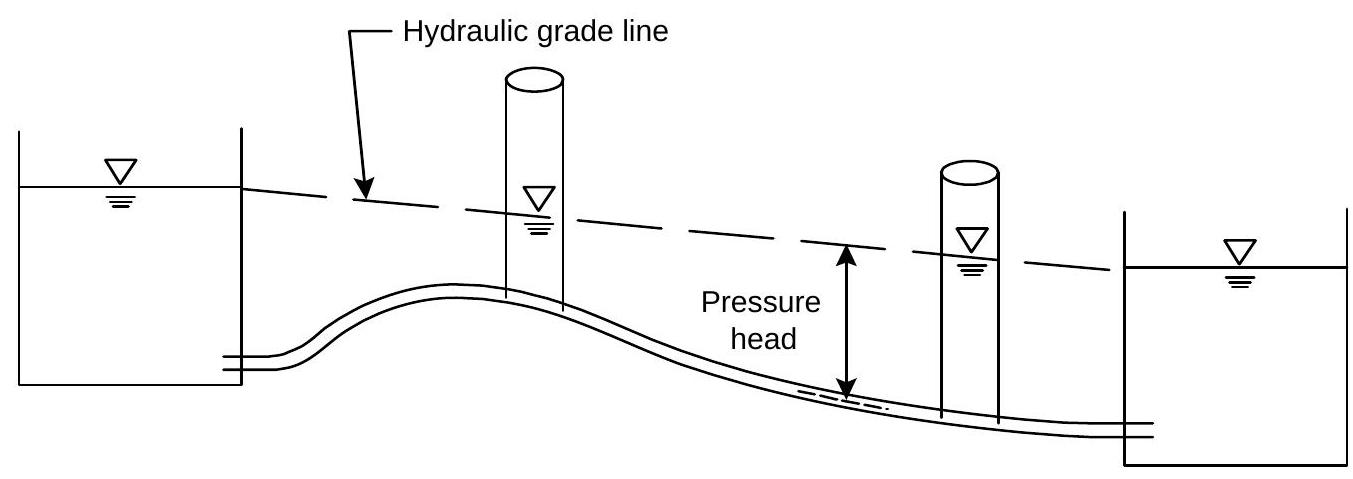
\includegraphics[max width=\textwidth]{2022_10_30_098bb5f44c5986ff92a9g-30}

Figure $2.18$ - Hydraulic Grade Line

\section{Energy Loss}
The difference between the Hydraulic grade line at two different points, one up stream the other downstream, equals energy loss. Energy Loss, or headloss, can have a negative impact on system pressures and flows.

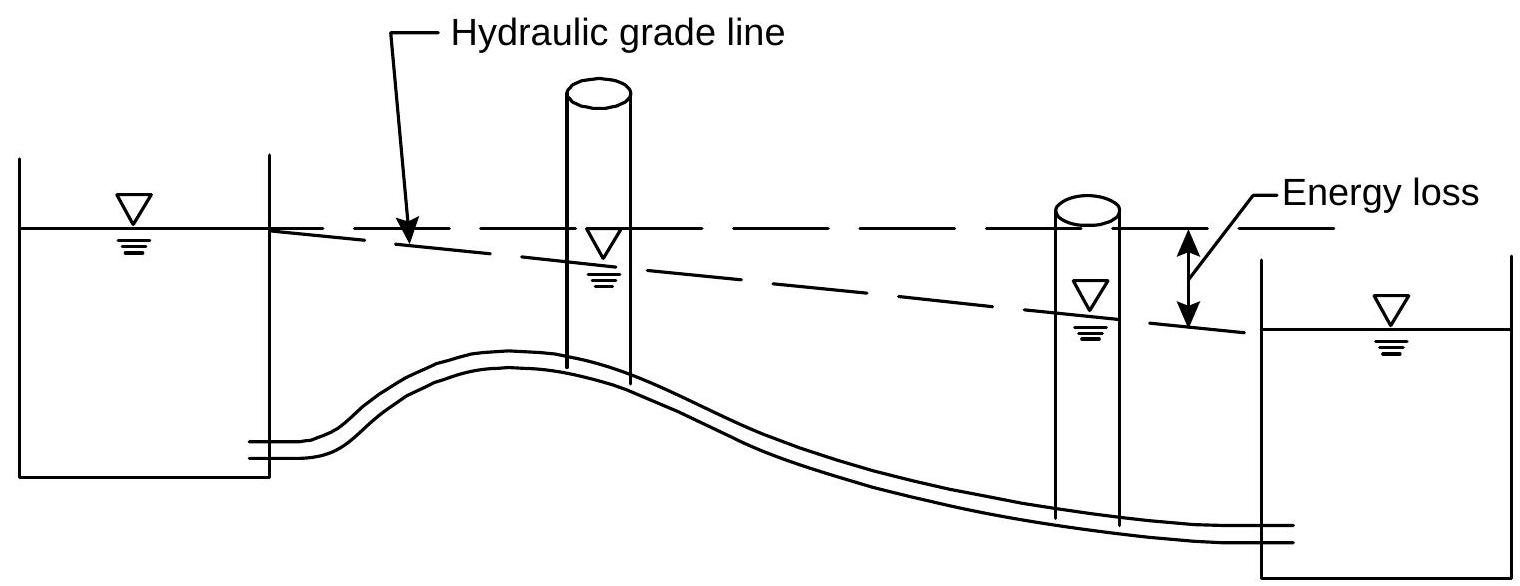
\includegraphics[max width=\textwidth]{2022_10_30_098bb5f44c5986ff92a9g-31}

Figure $2.19$ - Energy Loss

\section{Friction Losses}
$\square \quad$ Water will flow downhill with no problem. But there is friction between the water and the inside surface of the pipe.

As water travels through a pipeline, the energy or head of the water is reduced as turbulence in the water increases due to friction created by the roughness of the pipe walls.

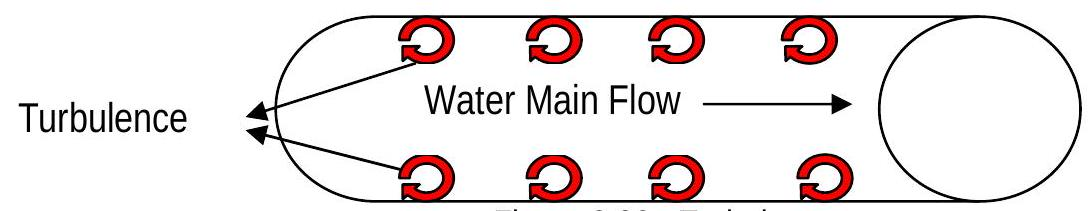
\includegraphics[max width=\textwidth]{2022_10_30_098bb5f44c5986ff92a9g-31(1)}

Figure $2.20$ - Turbulence

If the inside of the pipe is extremely rough, there is more friction loss between the water and the pipe.

Friction loss in a pipe depends upon the velocity or rate of flow and the size of the pipe (diameter), the length of the pipe, and the roughness of the inside surface of the pipe.

The degree of pipe roughness is called the $\boldsymbol{C}$-Factor. The $\boldsymbol{C}$ value is derived by using the Hazen-Williams equation which relates the flow of water in a pipe with the physical properties of the pipe and the pressure drop caused by friction. The lower $\boldsymbol{C}$ values represent smoother inside surfaces of the pipe.

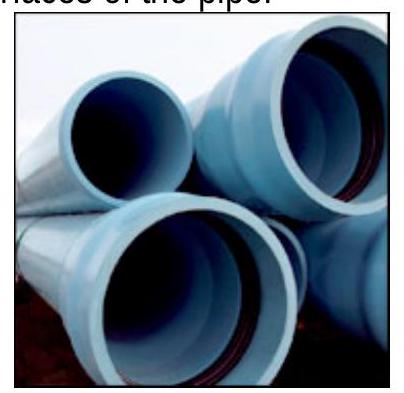
\includegraphics[max width=\textwidth]{2022_10_30_098bb5f44c5986ff92a9g-32}

The pipeline roughness varies based on the age, material, size of the pipeline, and the quality of the water that flows through the pipeline.

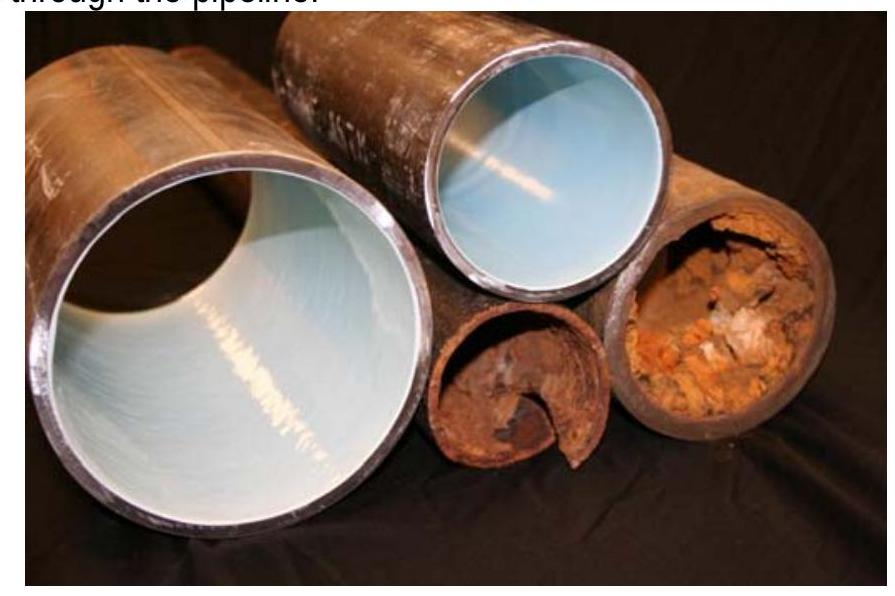
\includegraphics[max width=\textwidth]{2022_10_30_098bb5f44c5986ff92a9g-32(1)}

Tuberculation in the pipes can cause a substantial increase in friction loss, and can also significantly reduce the effective diameter of a pipe. This loss in diameter decreases the carrying capacity of the pipe as well as reduces the available pressure in the pipeline.

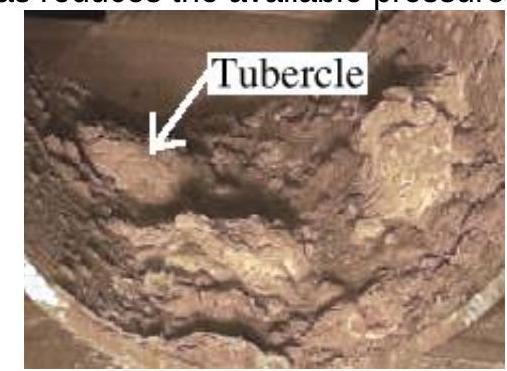
\includegraphics[max width=\textwidth]{2022_10_30_098bb5f44c5986ff92a9g-32(2)}

A general rule of thumb to estimate headloss is that it is approximately equal to the flow in a pipeline, squared. Therefore, if the flow in a pipeline is doubled, the headloss will increase by a factor of about 4.

\section{Minor Losses}
Headloss caused by rapid changes in velocity due to:

\begin{itemize}
  \item Changes in pipe diameter, shape, or direction, or

  \item Meters and valves.

\end{itemize}
\section{Customers and Demands}
\section{Terms and Definitions}
Consumption-refers to actual (metered) or estimated water uses within a distribution network. Consumption includes metered or estimated customer usage and can also include authorized uses that can be estimated such as fire fighting, main flushing, and street cleaning.

Unaccounted-for Water- is the difference between the amount of water produced and the amount of water metered for billing purposes. It generally refers to water used or lost from the distribution network that cannot be estimated such as water lost through main breaks or leaks, inaccurate meters, or theft of water. Other examples may be sites that never had meters installed such as libraries, schools, and churches.

System Demand-is the total amount of water supplied to the system, including consumption and unaccounted-for water. System demand is commonly referred to in units of gallons per day (gpd).

\section{Customer Types}
Customers of a water system are often classified by category for record keeping purposes. Typical customer category types are as follows:

Residential customers include residential or domestic establishments. Residential customers can also include apartment complexes and mobile home parks.

Commercial customers include typical commercial businesses, including stores and office buildings.

Industrial customers include larger facilities such as industrial plants and warehouses.

Other commonly used customer category types include institutional (schools, hospitals, etc.), bulk (service to another water utility), and municipal (municipal buildings and facilities).

\section{Diurnal Demands and Peaking Factors}
System demands vary throughout the course of a day and on a day-to-day basis. The Diurnal Demand Curve below illustrates the typical fluctuations in demand throughout a given day.

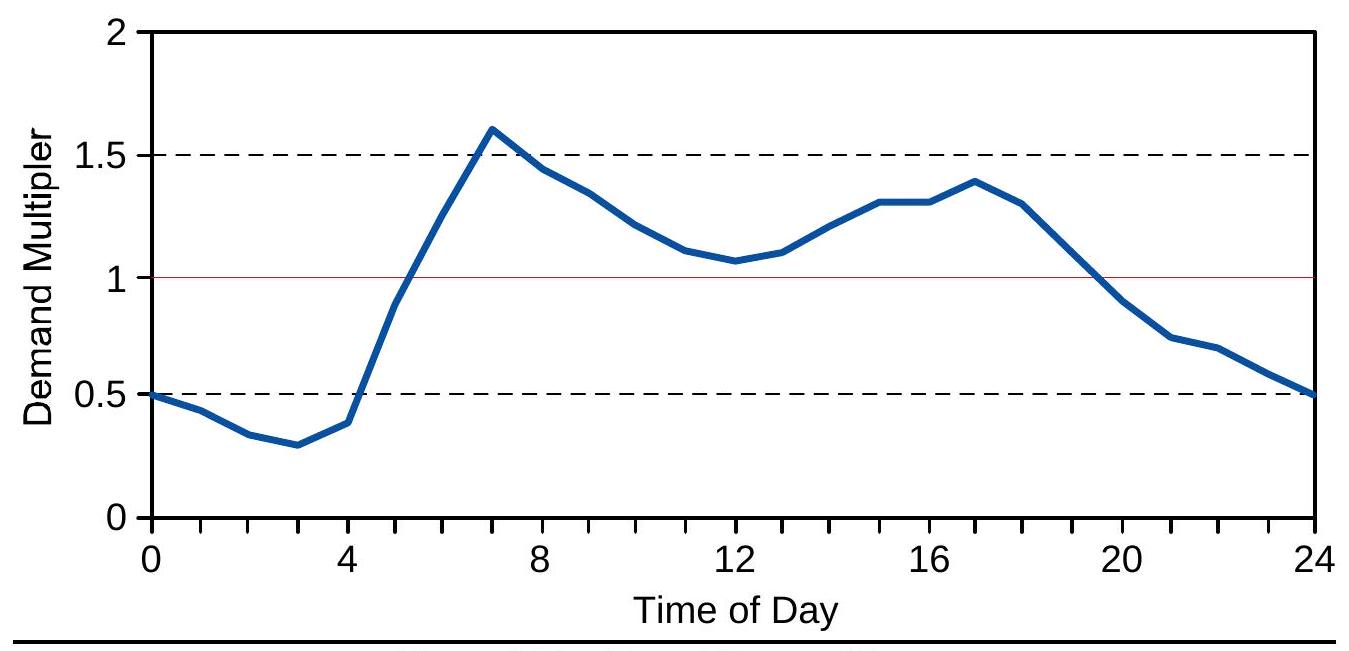
\includegraphics[max width=\textwidth]{2022_10_30_098bb5f44c5986ff92a9g-34}

Figure $2.21$ - Diurnal Demand Curve

Demands are usually relatively low during the night when most people are sleeping compared with demands in the early morning hours when people wake and prepare for the day.

Summer demands are usually relatively high compared to demands in the winter due to additional summer water uses such as irrigation.

Distribution network components are typically sized to meet these peak demands.

As the flowrate in distribution network pipelines varies due to variations in system demand, the HGL and pressures in the system will vary due to increases and decreases in system headloss. The variations in system demand will also result in variations in the water level of storage facilities, which will affect the system $\mathrm{HGL}$ and pressures.

A system is comprised of primarily residential customers. What are some trends that you could expect with regard to seasonal demands and diurnal demand patterns?

How will pressures likely be affected with these variations in demand?

If the system is comprised of primarily industrial users, would you expect similar variations in demands?

\section{Pressures}
\section{Pressures and Flows}
Adequate positive pressure should be provided throughout a distribution network to ensure adequate water service and protect the system against backflow. The main purpose of elevated tanks in water distribution systems is to boost the pressure in the system.

Normal pressures should generally range from a minimum of approximately 35 psi to a maximum of approximately 100 psi. The minimum pressure allowed in a distribution system is 20 psi. When pressures drop below 20 psi, a system could experience backflow conditions which could impact water quality.

Often when a water system service area has a wide range of ground elevations within its boundaries, water distribution networks are comprised of several pressure zones to provide acceptable pressures to the varying ground elevations.

$\square$ Pressure zones are typically separated by pumps, pressure control valves, and isolation valves.

\section{Flows}
Water distribution network pipelines are generally sized to meet peak demands, including fire flows.

Fire flow needs vary throughout a distribution network based on the types of customer facilities in a given area.

Fire flow needs typically range from a minimum of 500 gallons per minute (gpm) for low density residential areas to $3,500 \mathrm{gpm}$ or more for areas with large or high occupancy facilities.

\section{Surge in Pipelines}
Rapid changes in flow velocity within a distribution network can result in a pressure surge or water hammer. If not properly controlled, the pressure surge can result in failure of distribution network components.

Potential Problems

\begin{itemize}
  \item Pipe bursting,

  \item Pipe collapsing, or

  \item Failure of other distribution network components.

\end{itemize}
Possible Causes

\begin{itemize}
  \item Opening or closing valves too quickly.

  \item Starting or stopping pumps, or

  \item Opening or closing fire hydrants too quickly.

\end{itemize}
\section{Preventative Measures}
\begin{itemize}
  \item Proper operations, including slow opening and closing of valves and hydrants.

  \item Use of pressure surge control devices such as pressure and surge relief valves, vacuum relief valves, and surge tanks.

\end{itemize}
Customers in a large, new residential development are complaining of inadequate pressure. The development is served by 2-inch main. The water company installed a pressure gauge and determined that the typical pressure in the development is approximately 10 psi. Do the customers have a valid complaint? If yes, what can be done to resolve the problem?

\section{Routine Maintenance}
There are five programs involved in the routine maintenance of distribution networks. They are Pump Maintenance, Valve Maintenance, Meter Testing and Maintenance, Fire Hydrant Maintenance, and Inspection and Monitoring.

\section{Pump Maintenance}
Every system should have a regular program to inspect and maintain pumps.

\begin{itemize}
  \item Clean the pump and motor

  \item Check condition of impeller, bearings, seals and alignment of couplings.

  \item Visual inspection for excessive noise, vibration, heat and odor.

  \item Consult manufacture for complete list of maintenance items and methods.

\end{itemize}
\section{Valve Maintenance}
All distribution network valves require regular maintenance, including:

Routine inspections and exercising of valves, at least once per year, to ensure proper function and extend the life of the valve. Inspections should include verification of actual valve location according to system maps and/or intersection details. All valves should be numbered for easy identification.

\begin{itemize}
  \item Verify the accuracy of the location of the valve boxes on the system map and update map where necessary.

  \item Remove valve box cover and inspect stem and nut for damage or obvious leakage. - Close the valve fully and record the number of turns to the fully closed position (always close slowly to prevent water hammer).

  \item If possible, use leak detection tool like a ground microphone to determine if the valve is closed.

  \item Record condition of the valve and if any maintenance is required. An example valve operation worksheet is on page 2-28.

  \item Clean the valve box cover seat.

  \item Replace any missing valve box covers.

  \item Place the valve in its operating position (open or closed) when inspection is complete.

  \item To ensure the valve is placed back in its proper position (open or closed) a good method is to use spray paint. When you close the valve, paint a "C" on the ground around the box, when you open the valve, paint the rest of the "C" and make it look like an "O".\\

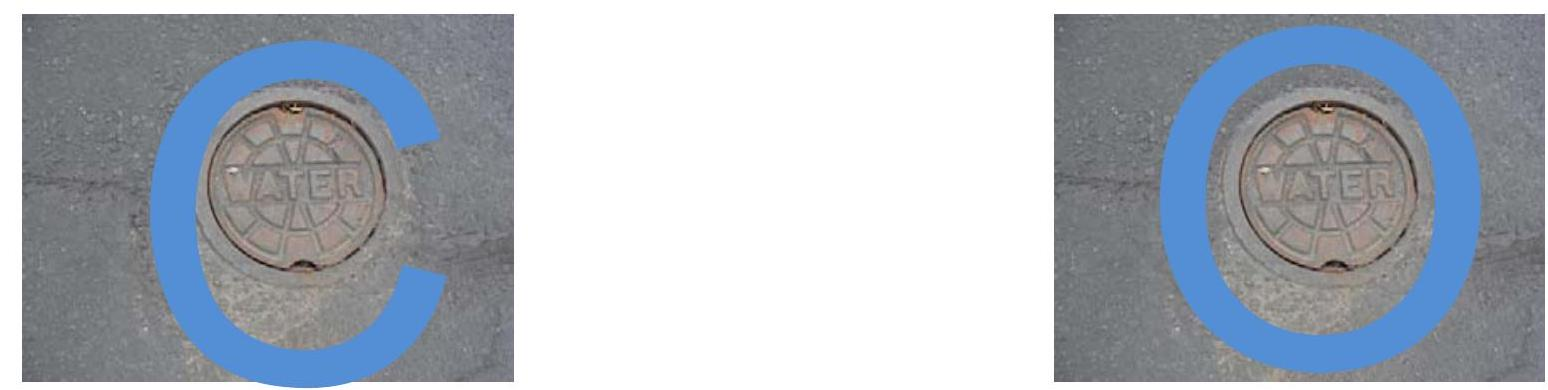
\includegraphics[max width=\textwidth]{2022_10_30_098bb5f44c5986ff92a9g-37}

\end{itemize}
Other valves in a distribution system need maintenance too.

Automatic air release, vacuum breaker, or pressure-reducing valves should be inspected at least every six months. These valves usually have an O\&M manual, which describes how they are to be inspected and maintained. Manual air releases should be opened and flushed to remove accumulated air, at least twice per year.

Additional details regarding proper operation and maintenance of valves can be found in Key Criteria for Valve Operation and Maintenance, and Guidance for Management of Distribution System Operation and Maintenance, AWWA Research Foundation.

\section{Valve Operation Worksheet}
\section{Operator}
\begin{tabular}{|l|l|l|l|l|l|l|}
\hline
Date & Valve No & Location & Size & \#of Turns & Direction of Closing & Remarks/Maintenance/Deficiencies \\
\hline
 &  &  &  &  &  &  \\
\hline
 &  &  &  &  &  &  \\
\hline
 &  &  &  &  &  &  \\
\hline
 &  &  &  &  &  &  \\
\hline
 &  &  &  &  &  &  \\
\hline
 &  &  &  &  &  &  \\
\hline
 &  &  &  &  &  &  \\
\hline
 &  &  &  &  &  &  \\
\hline
\end{tabular}

\section{Meter Testing and Maintenance}
The accuracy of a water meter may decrease over time due to wear, water deposits, or turbulence.

Periodic testing helps ensure accurate readings and limit lost revenues resulting from underregistering meters.

When establishing a meter testing program, the following issues should be considered:

\begin{itemize}
  \item Age of meter,

  \item Water use, and

  \item Water quality.

  \item Cost of testing and/or replacing meters.

\end{itemize}
Test procedures vary based on meter type and can be obtained from the meter manufacturer.

\section{Fire Hydrant Maintenance}
Annual Inspection and Operation

Can be performed efficiently in conjunction with pipe flushing.

Inoperative hydrants should be noted and tagged.

\section{Inspection and Monitoring}
Routine inspection and maintenance of the distribution network should include:

Daily inspection of key components such as storage and pumping facilities.

Make sure that hatches and gates are locked.

Access to distribution network components should be restricted to water system personnel only.

\section{Pipeline Maintenance}
There are three key components of a pipeline maintenance program. They are Leak Detection, Main Break Repair and Replacement, and Cleaning and Lining.

\section{Leak Detection}
Common methods of leak detection include:

Direct observation,

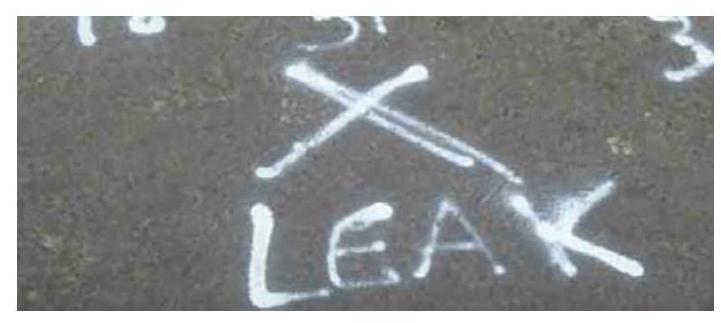
\includegraphics[max width=\textwidth]{2022_10_30_098bb5f44c5986ff92a9g-40}

Use of acoustic equipment e.g. geophones, devices using amplifiers to boost sound such as ground mikes, and other listening devices, and correlators to help pinpoint leaks.

Water audits.

\section{Main Break Repair and Replacement}
Main breaks are caused by unbalanced forces exerted on a pipeline, which may result from events such as subsidence, earthquake, and freeze/thaw cycles.

Detection of Main Breaks

\begin{itemize}
  \item Physical observations.

  \item Customer complaints of low pressure.

  \item Observation of non-typical system records.

\end{itemize}
Main Break Response Steps

\begin{itemize}
  \item Locate the leak.

  \item Notify PA. ONE CALL (811)

  \item Make preliminary assessment of the situation, including identifying procedures to isolate the break and the corresponding effects on pressures, and impacts to affected customers. The minimum pressure in a distribution system should be no less than $20 \mathrm{psi}$ at all times to prevent back-flow or back siphonage.

  \item Isolate the leak.

  \item Make full assessment of the situation, including traffic control, and safety procedures required such as shoring, evacuation routes, finalizing the repair method, and inspections. - Remember, any excavation over 5 feet deep requires shoring to insure the safety of personnel entering the trench.

  \item Once the break is exposed, the determination of the best repair method is made. Some smaller repairs will require clamps which cover the affected area. Other breaks, such as horizontal splits in lengths of pipe will require replacing the length of pipe.

  \item To minimize the risk of contamination, consider making repairs under system pressure with the water flowing.

  \item If the repair includes bends where thrust block have been used, thrust blocks should again be utilized. Their purpose is to prevent pipe movement due to pressure surges.

  \item Repair and test, including disinfection, and flushing.

  \item Return main to service and restore site.

  \item Develop a main break report.

\end{itemize}
Water Main Replacement

\begin{itemize}
  \item Reports and records of main breaks should be used to assist in prioritizing water main replacements. Areas where main breaks are a regular occurrence should be scheduled for replacement.

  \item When replacing sections of main line, make sure to utilize all the required safety precautions.

  \item Any excavation over 5 feet deep requires shoring to be used. If the trench is long enough to warrant it, safety ladders for exiting the trench should be no more than 25 feet apart.

  \item If multiple lengths of pipe are to be replaced, make sure the new pipe is inspected to be free of debris before it is inserted. Be sure the new pipe is properly placed. For example, bell-and-spigot piping normally has marks indicating the proper insertion depth on each length. This prevents movement of the pipe once the system is pressurized.

  \item If gaskets are used, make sure the gaskets are properly placed so they are not twisted or chipped. Another tool for preventing pipe movement is thrust blocks. They are placed on bends where pressure surges might cause the pipe to move.

  \item The trench should be refilled appropriately. The bedding around the pipe should be of uniform size and material. Allowing materials of various sizes such as large rocks could cause the pipe to fracture during settlement. Backfill material should be compacted at one foot intervals to minimize settlement.

  \item Once the trench is refilled, follow the disinfection, pressure testing, flushing and bacteriological procedures as discussed in basic main installation.

\end{itemize}
\section{Cleaning and Lining}
Cleaning and lining of water mains is performed to improve water quality and increase the hydraulic capacity of pipelines. These can result in increased flows and pressures and reduction of pump power costs.

\section{Key Points for Unit 2 - Distribution Networks}
\begin{itemize}
  \item Drinking water distribution networks provide adequate supplies of safe drinking water and fire flows to areas of the system.

  \item Transmission systems typically have large diameter pipes and no direct connections to customers.

  \item Distribution storage tanks help offset system demand fluctuations.

  \item Typical pump efficiencies can vary from 50 to 85 percent depending on the size and characteristics of the pump.

  \item Valves are used to isolate sections of water mains and to control flow and pressure.

  \item Dry barrel hydrants are used to prevent damage from freezing.

  \item Backflow protection helps to keep harmful contaminants from entering the distribution network.

  \item Unaccounted-for-water is the part of the total water produced that is lost from the distribution network and cannot be explained by main breaks, leaks, inaccurate meters or theft of water.

  \item Diurnal water demand curves usually show a peak demand for the water in the morning and in the evening.

  \item Normal water pressures in a distribution system usually range from 35 psi to 100 psi. The minimum allowable pressure is $20 \mathrm{psi}$.

  \item The proper sequence for replacing lengths of main line is disinfect, pressure test, flush and bacteriological testing. The new line can be placed into service after good bacteriological results are obtained.

\end{itemize}
\section{Unit 2 Exercise}
\begin{enumerate}
  \item Circle those items that are components of a distribution network.\\
a. Pumps\\
c. Storage Facilities\\
d. Intake\\
f. Pipes\\
g. Hydrants\\
h. Valves\\
j. Meters
\end{enumerate}
\section{Trench Safety fill in the blank}
\begin{enumerate}
  \setcounter{enumi}{2}
  \item OSHA requires a protective system for trenches feet or greater.

  \item Atmospheres containing oxygen levels below may be hazardous.

  \item A stairway, ladder, ramp or other safe means of egress shall be located in trench excavations that are feet or more in depth so as to require no more than feet of lateral travel for employees.

\end{enumerate}
\section{New main installation fill in the blank}
\begin{enumerate}
  \setcounter{enumi}{5}
  \item 
  \begin{itemize}
    \item the portion of the material placed in an excavation on either side of and under a pipe from the top of the bedding up to the springline or horizontal centerline of the pipe. This backfill layer extends from one trench sidewall to the opposite sidewall. This is the most critical area in providing support for a pipe.
  \end{itemize}
  \item To minimize settling, during a backfill operation, it is recommended that after every inches of lift, material should be compacted.

  \item The 4 crucial steps that are necessary before putting a new main in service:

  \item 
  \item 
  \item 
  \item 
\end{enumerate}
\section{$\underline{\text { Valve Matching }}$}
Use word bank to fill in the blanks in 8 through 13

Butterfly valve

Altitude valve Gate valve

Check valves Pressure Reducing valve

Air release valves

\begin{enumerate}
  \setcounter{enumi}{8}
  \item are used in distribution systems to prevent

  \item are used to create headloss and "break" pressure to keep system pressures less than the pressure ratings in pipes and to avoid other adverse impacts of high pressure.

  \item are the most commonly used isolation valve.

  \item are a flow control valve that can be adjusted to allow various flows through piping.

  \item are used to eliminate air from a distribution network or to allow air into a distribution network.

  \item is a type of valve used to control flow in and out of storage facilities based on water level.

  \item Corporation stops are typically tapped at:

\end{enumerate}
\section{Random Multiple Choice}
a. 10:00 o'clock position\\
b. 11:00 o'clock position\\
c. 12:00 o'clock position\\
d. 1:00 o'clock position

\begin{enumerate}
  \setcounter{enumi}{15}
  \item Rapid changes in flow velocity within a distribution network can result in:\\
a. Water hammer\\
b. Pipe bursting\\
c. Failure of distribution network component\\
d. All of the above

  \item Commonly used as a customer service meter:\\
a. Velocity\\
b. Compound\\
c. Displacement\\
d. Proportional 17. A flow of\\
a. Below $500 \mathrm{gpm}$\\
b. $500-9999 \mathrm{gpm}$\\
c. $1000-1499 \mathrm{gpm}$\\
d. $1500 \mathrm{gpm}$ or more can easily be identified if the top of the hydrant is painted blue.

  \item The pressure gauge at the bottom of the tank reads 12 psi. How many feet of water would you expect in the tank?\\
a. About 2 feet\\
b. About 5 feet\\
c. About 28 feet\\
d. About 60 feet

  \item Thrust blocks or restraints should be used at\\
a. Tees\\
b. Bends\\
c. Hydrants\\
d. All of the above to avoid movements and leaks:

  \item List the five programs involved in routine maintenance of distribution networks.\\
a.\\
b.\\
c.\\
d.\\
e. 1 "Fastite Joint Pipe" - \href{http://www.acipco.com/adip/pipe/fastitelindex.cfm}{www.acipco.com/adip/pipe/fastitelindex.cfm}. (16 Jun. 2003).

\end{enumerate}
2 "Mechanical Joint Pipe” - \href{http://www.acipco.com/adip/pipe/mechanical/index.cfm}{www.acipco.com/adip/pipe/mechanical/index.cfm}. (16 Jun. 2003).

3 "Flanged Pipe" - \href{http://www.acipco.com/adip/pipe/flanged/index.cfm}{www.acipco.com/adip/pipe/flanged/index.cfm}. (16 Jun. 2003).

4 "MJ Coupled Joint" - \href{http://www.acipco.com/adip/pipe/restrained/mj.cfm}{www.acipco.com/adip/pipe/restrained/mj.cfm}. (16 Jun. 2003).

5 "F-503 Gate Valve" - \href{http://www.wattsreg.com}{www.wattsreg.com} (16 Aug 2004)

6 “CLA-VAL model 90-01/690-01” - \href{http://www.cla-val.com}{www.cla-val.com} (16 Jun. 2003).

7 "CLA-VAL series 34 Air Release Valve" - \href{http://www.cla-val.com}{www.cla-val.com} (16 Jun. 2003).

8 "T-10 Meter sizes 11/2" and 2"' - \href{http://www.neptunetg.com}{www.neptunetg.com} (16 Jun. 2003).

9 "Cold Water Recordall ${ }^{\circledR}$ Turbo 2000 Meter" - \href{http://www.badgermeter.com/pdf/recturbo/tech/}{www.badgermeter.com/pdf/recturbo/tech/} rts-t-6.pdf (16 Jun. 2003).

10 "Cold Water Recordall ${ }^{\circledR}$ Combo Meter" - \href{http://www.badgermeter.com/pdf/recomp/tech/rcm-t-08.pdf}{www.badgermeter.com/pdf/recomp/tech/rcm-t-08.pdf} (16 Jun. 2003).

11 "Magnetoflow ${ }^{\circledR}$ Mag Meter model Magnetoflow ${ }^{\circledR}$ Flanged" - \href{http://www.badgermeter.com/pdf/}{www.badgermeter.com/pdf/} indust/ primo/ itb-106.pdf (16 Jun. 2003).

12 "HP Protectus III Fire Service Meter - Sizes 4", 6", 8" and 10"' - \href{http://www.neptunetg.com/}{www.neptunetg.com/} default.cfm?doc\_id=8 (16 Jun. 2003).

13"The Case for Inspecting Fire Hydrants" - \href{http://www.muellercompany.com/files/11735%209-10.pdf}{www.muellercompany.com/files/11735 9-10.pdf}. (5 Jun. 2013)

\section{Additional Resources Used}
Thomas Walski, Donald V. Chase, Dragan Savic, Walter M. Grayman, Stephen Beckwith, and Edmundo Koelle, "Advanced Water Distribution Modeling and Management," (Haestad Methods, Waterbury, CT: Haestad Press, 2002) p. 135, 151-157, 165-166, 573-574, 602-614.

"Community Water Systems," Public Water Supply Manual, (PA DEP) Part II 7.0.18, Part IV $1.1$.

"Distribution Components and Disinfection Student Manual," (PA Rural Water Association, Bellefonte, PA: PRWA) p. 3-6, 9-13, 15-35. "Guidance for Management of Distribution System Operation and Maintenance," American Water Works Association Research Foundation \#2, (AWWA Research Foundation, Denver, CO: AWWARF) p. 30$43,64-65,70-75$.

"Guidance Manual for Monitoring Distribution System Water Quality," AWWA Water Distribution System Operation and Maintenance, (AWWA Denver, CO: University of California at Sacramento) p. 2.0, $2.1,2.31,2.35,2.41,2.42,3.0,3.3,3.4,3.5,3.61,3.62,3.63,3.64,3.670,3.671,3.672,3.7,3.8,3.83,5.1$, $5.4,5.6,5.700,5.701,5.706,5.707,5.708,5.71,5.72,5.73$,and $5.74$.

"Key Criteria for Valve Operation and Maintenance," American Water Works Association Research Foundation \#1, (AWWA Research Foundation, Denver, CO: AWWARF) p. 2.2.1, 2.2.4, 3.5, 4.5.2, and 5.

"Manual of Water Supply Practices," American Water Works Association M32 Distribution Network Analysis for Water Utilities, (AWWA Denver, CO) p. 44-47.

"Prioritizing Water Main Replacement and Rehabilitation," American Water Works Association Research Foundation \#3 Appendix A, (AWWA Research Foundation, Denver, DO) p. 103-105.

"Research Foundation," American Water Works Association Research Foundation \#4, (AWWA Research Foundation, Denver, CO: AWWARF) p.61-67, 65-70, 75-82, 89-93, 96-99.

"Wastewater Treatment Plant Operator Training Module 9: Basics of Pumps and Hydraulics," (PA DEP Bureau of Water Supply and Wastewater Management) (30, Jun. 2003).

\section{Unit 3 - Distribution Storage}
\section{Learning Objectives}
\begin{itemize}
  \item List the three primary functions and identify the four types of distribution storage facilities.

  \item Calculate the volume of water in a storage facility and define the components of distribution system storage volume allocation.

  \item Explain the procedures and methods utilized in controlling the filling and draining of distribution storage facilities.

  \item $\quad$ State three primary maintenance issues or concerns involved with distribution storage facilities.

\end{itemize}
\section{Purpose of Distribution Storage}
\section{Purpose}
The three primary functions of distribution storage facilities are as follows:

Equalize Demands

\begin{itemize}
  \item One of the primary purposes for constructing a storage facility is equalization.

  \item Water utilities like to operate treatment plants at a relatively constant rate however water use in most utilities varies significantly over the course of a day.

  \item Distribution storage facilities are typically designed to offset fluctuations in system demands, thus allowing a more constant rate of flow from the source of supply.

\end{itemize}
Minimize fluctuation in system pressure

\begin{itemize}
  \item Generally, the elevation of water stored in a tank determines the pressure in pipes which are directly connected to the tank.

  \item The larger the tank volume, the more stable the pressures in the distribution system despite fluctuations in demand or changes in pump operation.

  \item This type of design helps minimize capacity requirements of sources of supply, treatment facilities, and transmission and distribution mains, minimize fluctuations in system pressures, and increase distribution pumping efficiency.

\end{itemize}
$\square \quad$ Fire Protection

Distribution storage facilities are used to help meet fire flow needs in systems that provide fire protection.

\section{Emergency Supply}
Distribution storage facilities provide a volume of water that can be used to supply a system or parts of a system during an emergency event such as pump failures or main breaks.

\section{Types of Storage Facilities}
The primary types of distribution storage facilities are as follows:

\section{Clear well}
Clear wells are often used for storage of treated water at a treatment facility. They can be constructed above or below ground. When they are below ground, they constitute a confined space. When operators are intending to clean a clear well which requires entering the confined space, all the usual safety requirements should be utilized. First, and foremost, the atmosphere should be vented and tested. As discussed, normal atmospheric oxygen levels are around $20 \%$. Safety harnesses and tripods should always be used, and an operator should never enter a confined space unless there are other workers involved.

\section{Elevated}
Elevated storage facilities are typically used to boost pressure in distribution systems

\includegraphics[max width=\textwidth]{2022_10_30_098bb5f44c5986ff92a9g-50}

Figure $3.1$ - Elevated Tank

\section{Ground Level}
Ground level storage facilities are storage facilities that are constructed at or below ground level. Ground level storage facilities are generally less expensive to construct and easier to maintain than elevated storage facilities. Occasionally, pumps are used to maximize the useable storage volume in ground level storage facilities.

\includegraphics[max width=\textwidth]{2022_10_30_098bb5f44c5986ff92a9g-50(1)}

Figure $3.2$ - Ground Level Tank Stand pipe

If the tank is significantly taller than it is wide, it is usually referred to as a standpipe.

\includegraphics[max width=\textwidth]{2022_10_30_098bb5f44c5986ff92a9g-51}

Figure $3.3$ - Stand Pipe

\section{Hydropneumatic}
Hydropneumatic or pressure tanks are typically used in smaller systems or small sections of a system that do not have elevated or ground level storage. Hydropneumatic tanks are used to regulate and maintain water pressure and promote more efficient pump operations in these areas. Pressure in a hydropneumatic tank is controlled by the volume of air in the tank relative to the volume of water.

\includegraphics[max width=\textwidth]{2022_10_30_098bb5f44c5986ff92a9g-51(1)}

Figure $3.4$ - HydropneumaticTank ${ }^{1}$

\section{Storage Volume and Water Level}
\section{Volume Calculations}
The volume of water in a storage facility can be calculated for any given water level, if the dimensions of the tank are known. Tank volumes are typically provided in gallon units.

Volume Calculations for rectangular shapes:

Volume $(V)=$ Length $(I) \times$ Width $(\mathrm{w}) \times$ Height $(\mathrm{h})$,

or it can also be written as Volume $(V)=\operatorname{Area}(A) \times$ Height $(h)$,

and often written as: $\quad V=A \times H$

\section{Example $3.1$ - Volume Calculation}
A rectangular ground level storage facility is 100 feet long by 50 feet wide. The water level in the tank (measured from the bottom of the tank) is 10 feet. What is the volume (in gallons) of water in the tank?

\section{Example $3.2$ - Volume Calculation}
An elevated tank has a diameter of 50 feet. The water level in the tank is 20 feet. What is the volume of water in the tank? Another example of distribution "storage" is the volume of water contained in the pipes themselves. The volume of water in a pipe can be calculated using the same formula as above:

vol $=(0.785)(\text { dia })^{2}($ length $)\left(7.48 g a l / f{ }^{3}\right)$, substituting the length of pipe for the height of water

\section{Example $3.3$ - Volume Calculation}
How many gallons of water are in a 400 foot section of main that has an 8 inch diameter?

\section{Example $3.4$ - Volume Calculation}
The diameter of a tank is 60 feet. Without refilling of the tank, in one day, the water depth dropped from 25 feet to 21 feet, how many gallons of water were used that day?

\section{System Storage Allocation}
A combination of factors helps us determine the amount of water that must be stored. Projected needs for fire, emergencies and equalization all contribute to the determination.

\section{Useable Storage}
The useable storage is the total volume of water in a storage facility that can provide minimum required pressures to the highest elevation customers who are served by the facility. The useable volume of water in a storage facility is generally allocated for the three primary distribution storage functions previously described in this Unit.

\section{Equalization Storage}
Equalization storage provides storage for the equalization of system demands and pressures. It is designed to handle the normal daily fluctuations in water level in a storage facility due to peaks in system demand.

$\square \quad$ Fire Storage

A reserve volume of water to help meet system fire flow needs. The volume of fire storage needed is dictated by the maximum fire flow needs in the system.

Emergency Storage

A reserve volume of water to help meet system supply needs during an emergency event. The volume of emergency storage needed is typically dictated by system demands.

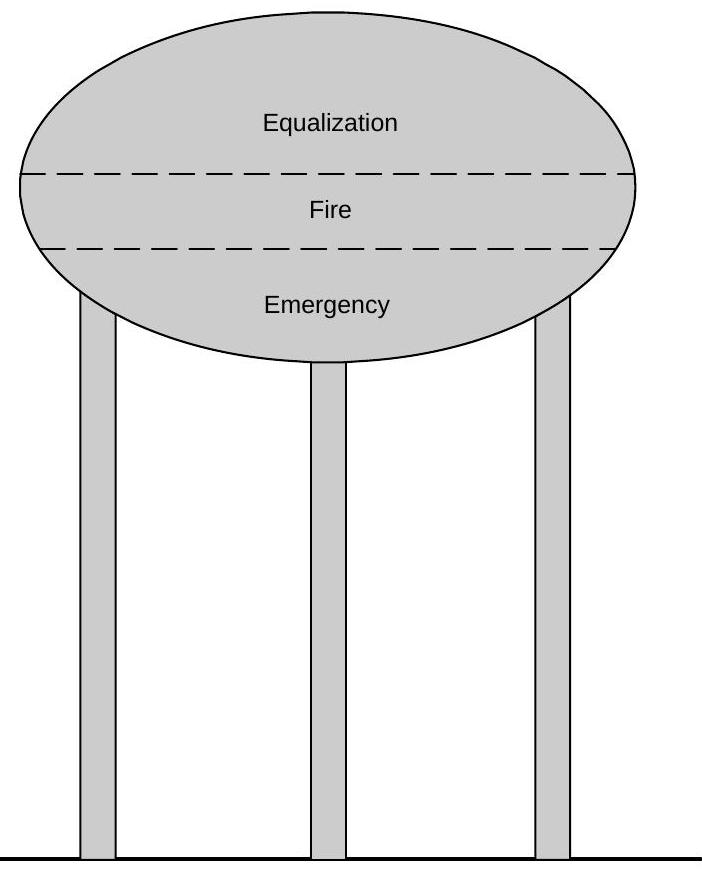
\includegraphics[max width=\textwidth]{2022_10_30_098bb5f44c5986ff92a9g-54}

Figure $3.5$ - Schematic for System Storage Allocation

\section{Operating Procedures}
\section{Refilling of Storage}
\section{Routine Refill}
The operation of distribution pumps is often controlled by the water level in a storage facility. When the water level in a storage facility reaches a set low level, the pumps are turned on until a set high level is reached. The operation of the distribution pumps and subsequent refilling of distribution storage can also be controlled by pressure, pump speed, flow rates, and time of day.

Many systems operate in a manner that allows pumping and subsequent refilling of storage facilities to occur during nighttime hours to minimize energy costs. This may not be feasible for certain systems due to the characteristics of a system, including demand patterns and available storage volume.

\section{Emergency Refill}
Secondary or lag pumps are typically operated to refill system storage following excessive peaks in demand or emergency conditions, such as a fire or a main break.

Procedures should be developed and utilized to manually or automatically control system facilities to ensure proper refill of system storage for normal and emergency conditions.

\section{Storage Level Controls}
Level Recorders

In order to maintain proper operations, the water level in a storage facility should be monitored and recorded at all times.

$\square \quad$ Control Valves

Altitude valves are used to control flow in and out of storage facilities and prevent overflows.

Altitude valves operate by sensing pressure. The pressure can be correlated to the water level in the tank using the formula provided in Unit 1.

Pressure, psi $=2.31 \times$ Head, $\mathrm{ft}$.

\section{Purpose of Maintenance}
Storage facilities require routine maintenance, including routine inspections, to ensure proper operation and identify replacement and repair needs.

\section{Painting}
\section{Frequency}
Inspections of the inside and outside of storage facilities are required to determine the need for repainting. Routine visual inspections of the inside of the storage facility could be made from the hatch of the facility. More detailed inspections of the interior require the facility be drained. These inspections should be conducted every several years depending on system conditions. Flaking, peeling, and rust are signs that repainting is needed. On average, typical storage tanks require repainting every 15 years.

\section{Painting Process}
When draining a tank for inspection or repainting, provisions should be made to ensure adequate system operation when the tank is out of service. The paint used must meet standards established by the Pennsylvania Department of Environmental Protection (PA DEP).

\section{Corrosion Control}
\section{Corrosion Influences}
Corrosion is a significant maintenance issue with storage facilities. Corrosion can occur on the inside or outside of a storage facility. Factors that contribute to increased risk of corrosion inside a tank include:

$\square \quad$ Warm water,

Long detention times (minimal turnover of water in a tank), and

Corrosive water (high in dissolved oxygen and sulfate, low in $\mathrm{pH}$ ).

\section{Corrosion Control Methods}
Methods of corrosion control include:

$\square$ Painting and routine repainting,

Coatings,

Cathodic protection, and

Addition of corrosion inhibitor as part of the water treatment process.

\section{Water Quality}
\section{Potential Water Quality Issues}
Degradation of water quality is another significant maintenance issue with distribution storage facilities. Three issues with storage facilities that can negatively impact water quality are described below.

\section{Excessive Detention Time}
In a storage facility, excessive detention time can result in depletion of chlorine residual. Excessive detention time occurs when adequate volumes of water are not transferred in and out of a storage facility on a routine basis. Excessive detention time can result from:

\begin{itemize}
  \item Low system demands;

  \item Improperly designed storage facilities; and

  \item Improper system operations.

\end{itemize}
\section{Contamination}
Water contamination in a storage facility can be caused by deliberate acts such as vandalism or terrorism, as well as by natural causes, such as animals or rain. Proper care should be taken to prevent contamination at storage facilities. This includes:

\begin{itemize}
  \item Restricting unauthorized access to storage facilities;

  \item Locking and sealing access openings; and

  \item Routine inspections and surveillance. Key Points for Unit 3 - Distribution Storage

  \item Drinking water storage distribution systems equalize demands and pressure fluctuations; provide fire protection and emergency stores of water.

  \item Storage facilities can be classified as clear wells, elevated, ground level and hydropneumatic.

  \item Routine refill is the normal schedule of restoring water levels to the desired amounts. Emergency refill is needed after excessive peak demand or emergency conditions.

  \item Painting and corrosion control methods can enhance the life of distribution storage facilities.

  \item Excessive detention time in a water storage facility can adversely affect water quality through depleted chlorine residual and increased chances of contamination.

\end{itemize}
\section{Unit 3 Exercise}
\begin{enumerate}
  \item List the three primary functions of distribution storage facilities.
\end{enumerate}
\begin{enumerate}
  \item 
  \item 
  \item 
\end{enumerate}
\begin{enumerate}
  \setcounter{enumi}{2}
  \item What are some advantages to using an elevated storage tank?

  \item Explain the procedures and methods used in controlling the filling and draining of a distribution storage facility that you are familiar with.

  \item List three maintenance issues concerning distribution storage facilities.

\end{enumerate}
\begin{enumerate}
  \item 
  \item 
  \item 
\end{enumerate}
\begin{enumerate}
  \setcounter{enumi}{5}
  \item A new section of 12 inch diameter pipe is to be disinfected before it is put into service. If the length of pipeline is 2000 feet, how many gallons of water will be needed to fill the pipeline? 1 "HydropneumaticTank" - \href{http://www.watertanks.com/images/pdf/watertankscom-gouldshydropro.pdf}{http://www.watertanks.com/images/pdf/watertankscom-gouldshydropro.pdf} (30 Jun. 2003).
\end{enumerate}
\section{Additional Resources Used}
"Community Water Systems," Public Water Supply Manual, (PA DEP) p.7.0.18.

"Distribution Components and Disinfection Student Manual," (PA Rural Water Association, Bellefonte, PA: PRWA) p. 30, 31, 32, 33, 34, 35.

"Guidance Manual for Monitoring Distribution System Water Quality," AWWA Water Distribution System Operation and Maintenance, (AWWA Denver, CO: University of California at Sacramento) p. 2.0, $2.1,2.31,2.41,2.42,3.4$

"Manual of Water Supply Practices," American Water Works Association M32 Distribution Network Analysis for Water Utilities, (AWWA Denver, CO) p. 44-47.

\section{Unit 4 - Water Quality and Monitoring}
\section{Learning Objectives}
\begin{itemize}
  \item Identify the three types of distribution system water quality issues.

  \item $\quad$ Describe the purpose of disinfection and chlorine residual in the distribution system.

  \item Identify the regulatory and non-regulatory water quality monitoring needs within a distribution system.

  \item List seven practices to enhance distribution system water quality.

\end{itemize}
\section{Purpose of Disinfection}
The use of chlorine in drinking water began in 1908 and shortly thereafter was called "a tremendous boon in the safeguarding of public health all over the world and is probably the most important and efficient sanitary measure of protection ever introduced ." $^{1}$ Today, chlorination of our water supplies is still used to protect the public's health. In fact, the Safe Drinking Water Act requires that all public water systems provide some type of disinfection and chlorination has remained the most common method of disinfection because of the easily detectable residual it leaves in the water. There are other methods of disinfection which include the use of ultraviolet light, iodine, bromide, and ozone. However, a chlorine residual must be maintained throughout the distribution system to help safeguard the distribution system by:

\begin{itemize}
  \item Protecting the distribution system from microorganisms

  \item Indicating distribution system upset; and

  \item Controlling biofilm growth

\end{itemize}
Treatment systems are required to monitor the chlorine residual throughout the distribution system. Ensuring chlorination in the distribution system is the last remaining barrier that prevents recontamination before the customer consumes the water and is a very crucial component of public health protection. In the event that a distribution check sample does not have a detectable chlorine residual:

\begin{itemize}
  \item A protocol should be in place which the operator should first consult.

  \item Next, the operator should notify the DEP as well as the public.

\end{itemize}
Maintaining a chlorine residual is not the only way a system protects public health. All public water systems are required to take bacteriological samples. In particular, we rely on monitoring our systems for coliform bacterial. Coliform bacteria are organisms that are present in the environment and in the feces of all warm blooded animals. The presence of coliform bacteria indicates that disease causing organisms (pathogens) could be in the water system. The number of bacteriological samples collected in the distribution system depends on the population served. The higher the population, the more coliform tests required. If a total coliform sample tests positive:

\begin{itemize}
  \item The lab will notify the system and

  \item The lab will run a fecal coliform and/or E-coli, and

  \item The lab will tell the system to grab check samples

  \item If the check samples test positive for coliform, they too will be checked for fecal or E-coli.

  \item In the event any sample tests positive for the fecal or E-coli,

  \item The system must issue a boil water advisory; and

  \item A Tier 1 Violation dictates DEP must be notified immediately

\end{itemize}
Note: A Tier 2 Violation of the MCL for total coliforms occurs when total coliforms are present in the water distribution system in either routine or check samples. For systems taking less than 40 samples per month, more than one positive sample per month constitutes a violation. For systems taking 40 or more samples per month, a violation occurs when more than five percent of the monthly samples taken test positive for total coliforms.

\section{Chlorination as a Disinfectant}
\section{Chlorine Reaction}
Chlorine $\left(\mathrm{Cl}_{2}\right)$ when injected into water forms the following reaction:
$$
\begin{array}{ccccc}
\mathrm{Cl}_{2}+\mathrm{H}_{2} \mathrm{O} & \Rightarrow & \mathrm{HOCl} & + & \mathrm{HCl} \\
\text { Chlorine }+\text { Water } \Rightarrow & \text { Hypochlorous Acid } & + & \text { Hydrochloric Acid }
\end{array}
$$
Chlorine is capable of disinfecting when in the "free residual" state. The two free residual forms of chlorine include:

Hypochlorous acid (HOCl), and

Hypochlorous Ion (OCL-).

Three forms of Chlorine Used

Calcium Hypochlorite

o Produced in tablet or granular form

o Contains about $65 \%$ available chlorine

o Often used in the disinfection of mains and storage facilities.

\section{Sodium Hypochlorite}
o Yellow/greenish liquid form of chlorine

o Generally contains about $10 \%$ or $12.5 \%$ available chlorine when purchased

o Some systems dilute with water depending on water flow and required dosage if used for system

\section{Gas Chlorine}
o If used, only used in treatment facility

$0100 \%$ strength

o Generally shipped in $150 \mathrm{lb}$ or ton cylinders

o Most dangerous of the three forms

\section{Depletion of Chlorine Residual}
Contributing Factors:

\begin{itemize}
  \item Inadequate disinfection of source,

  \item Stagnation/excessive detention time,

  \item Presence of ferrous ions and corrosion by-products in water, and

  \item Presence of bio-film and organic matter in mains and storage facilities.

\end{itemize}
Effects:

\begin{itemize}
  \item Biofilm growth, and

  \item Inadequate protection against bacteria that cause waterborne diseases.

\end{itemize}
\section{Disinfection Influences}
$\square \quad \mathrm{pH}$

$\square$ Temperature

$\square \quad$ Contact time

Concentration

Impurities in the water

\section{Breakpoint Chlorination}
As chlorine is added to water, it reacts with impurities in the water. The chlorine dosage needed to satisfy this initial chlorine demand of the impurities is referred to as breakpoint chlorination. Chlorine that is added beyond the breakpoint chlorination dosage is the free residual chlorine that is used for disinfection within the distribution system.

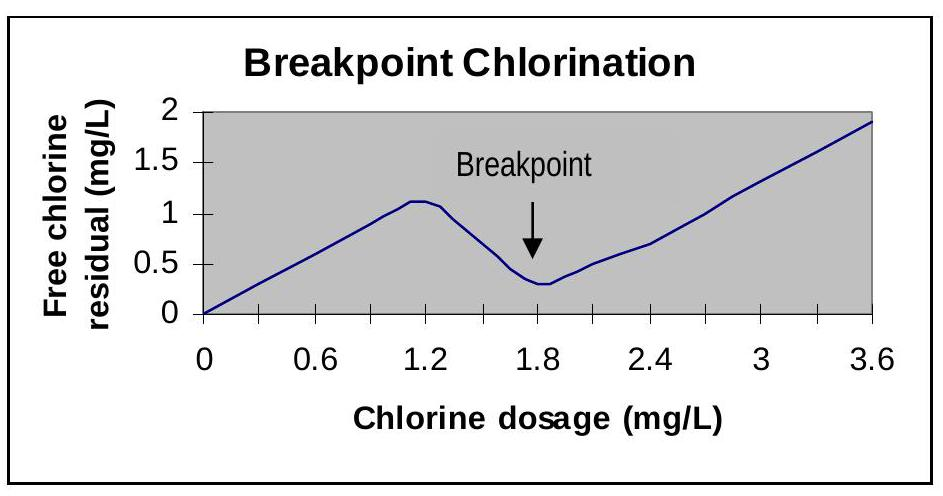
\includegraphics[max width=\textwidth]{2022_10_30_098bb5f44c5986ff92a9g-64}

Figure $4.1$ Breakpoint Chlorination

\section{Chlorine Dosage}
When analyzing chlorine residuals, the total chlorine is the total amount of chlorine that was added. This includes the amount needed for the chlorine demand and the free residual chlorine.

The required chlorine dosage is determined by adding the amount of chlorine it took to reach breakpoint chlorination and the amount of chlorine needed to hold the required residual for disinfection.

$\square$ This can be expressed:

\begin{itemize}
  \item $\quad$ Chlorine dosage $=$ Chlorine demand $+$ Chlorine residual.
\end{itemize}
\section{Example 4.1 - Dosage Calculation}
The chlorine residual is $0.7 \mathrm{mg} / \mathrm{l}$, and the demand is $0.5 \mathrm{mg} / \mathrm{l}$. What is the dose?

\section{Example 4.2 - Dosage Calculation}
The chlorine dose is $2.1 \mathrm{mg} / \mathrm{l}$, and the demand is $0.9 \mathrm{mg} / \mathrm{l}$. What is the residual?

Rearrange $=$ Chlorine Residual $=$ Chlorine Dosage $-$ Chlorine Demand

\section{Leaching of Coatings and Linings}
\section{Contributing Factors:}
\begin{itemize}
  \item New coatings or linings,

  \item Low pH, alkalinity, and calcium in cement and cement-lined mains and tanks, and

  \item Stagnation/excessive detention times.

\end{itemize}
\section{Effects:}
\begin{itemize}
  \item System contamination due to volatile organic compounds (VOCs) such as benzene, MBTE, and other contaminants,

  \item Increased nutrients and subsequent promotion of bacterial growth,

  \item Increased pH, calcium, and alkalinity (from cement lining),

  \item Taste, odor, and color issues, and

  \item Depletion of disinfectant residual.

\end{itemize}
\section{pH Instability}
Contributing Factors:

\begin{itemize}
  \item Low buffer capacity (inadequate alkalinity), and

  \item High alkalinity $(>1,000 \mathrm{mg} /)$ and $\mathrm{CaCO}_{3}(>50 \mathrm{mg} / \mathrm{l})$.

\end{itemize}
\section{Effects:}
\begin{itemize}
  \item Corrosion of distribution network components,

  \item Leaching of coatings and linings,

  \item Damage to cement and cement-lined mains and tanks, and

  \item Scale formation.

\end{itemize}
\section{Biological}
\section{Waterborne Diseases}
Contributing Factors:

\begin{itemize}
  \item Infiltration,

  \item Inadequate disinfection,

  \item Stagnation/excessive detention time,

  \item Presence of nutrients, and

  \item Presence of biofilm.

\end{itemize}
Effects:

\begin{itemize}
  \item Gastrointestinal diseases, when digested,

  \item Taste and odor issues, and

  \item Interference with microbiological monitoring.

\end{itemize}
\section{Biofilm}
Contributing Factors:

\begin{itemize}
  \item Corrosion and tuberculation,

  \item Temperature,

  \item Stagnation/excess detention time, and

  \item Presence of nutrients.

\end{itemize}
Effects:

\begin{itemize}
  \item Depletion of disinfectant residual,

  \item Taste and odor issues,

  \item Release of pathogenic organisms into the distribution system, and

  \item Interference with microbiological monitoring.

\end{itemize}
\section{Aesthetic}
Taste, Odor, and Color

Contributing Factors:

\begin{itemize}
  \item Inadequate treatment of metals, minerals, and VOCs,

  \item Presence of algae and microorganisms,

  \item Leaching of coatings and linings,

  \item High levels of disinfectant residuals,

  \item Corrosion and tuberculation,

  \item Infiltration, and

  \item Formation of air bubbles.

\end{itemize}
Effects:

\begin{itemize}
  \item Unpleasant appearance and taste,

  \item Customer complaints, and

  \item Staining can occur from precipitated iron and manganese in the distribution system.

\end{itemize}
\section{Sediment}
Contributing Factors:

\begin{itemize}
  \item Inadequate treatment,

  \item Sudden changes in flow velocity (scouring),

  \item Changes in flow direction,

  \item Corrosion and tuberculation,

  \item Infiltration, and

  \item Leaching of coatings and linings.

\end{itemize}
Effects:

\begin{itemize}
  \item Reduced pipeline hydraulic capacity,

  \item Taste, color, and odor issues,

  \item Growth of bacteria and biofilm, and

  \item Ineffective disinfection.

\end{itemize}
\section{Chlorine Residual}
\section{Disinfection of New Mains and Storage Facilities}
\section{New Mains}
\section{Contamination Prevention}
When installing water mains, care should be taken to prevent contamination from dirt, debris, animals, dirty water, or other potential contaminants. Mains should be plugged when unattended. Also, trenches should be kept clean and dry.

\section{Flushing}
New mains should be flushed at a rate of at least 5 feet per second for approximately 30 minutes to help remove potential contaminants. Flow is related to velocity as follows:
$$
\text { Flow }(\mathrm{Q})=\text { Velocity }(\mathrm{V}) \times \text { Diameter }(\mathrm{D})
$$

\section{Disinfection}
New mains should be disinfected prior to putting in service. Calcium hypochlorite in tablet or granular/solution form is often used for disinfecting new mains.

\section{Post-Disinfection}
The new main should be tested for coliform after disinfection to ensure the effectiveness of the disinfection. The main should be flushed again prior to putting it in service in order to remove the concentrated chlorine.

\section{Main Repairs}
The best way to make a system repair is to do it under system pressure with the water flowing. Contamination could occur when a main is removed from service for repairs. Thus, they should be flushed and disinfected after repairs, using similar procedures as described above for disinfection of new mains, prior to putting back in service.

\section{Storage Facilities}
New storage facilities and those removed from service for repair should also be disinfected prior to putting in service. Procedures for disinfection of a storage facility are similar to those for new mains. Disinfecting a storage facility could also be accomplished by filling the tank with water that has the appropriate chlorine residual. This can be accomplished by use of calcium hypochlorite at the tank.

\section{Disinfection Dosage Calculation}
To properly disinfect water mains, different methods can be applied. Typically, with regard to water mains and storage tanks, calcium hypochlorite in granular or tablet form is used. Typically, the pipe or tank is valved-off so that it can be filled with water for 24 hours. Determining how many pounds of calcium hypochlorite takes mathematical calculations.

\section{Example 4.3 - Dosage Calculation}
A system has replaced 200 feet of 8 inch water main. They are going to use $50 \mathrm{mg} / \mathrm{l}$ of chlorine for 24 hours to disinfect the line. How many pounds of $65 \%$ calcium hypochlorite are required?

You can use the feed rate formula to solve this, but first you need to determine the volume of water in the pipe. Use the formula for a volume of a cylinder (or circular tank)

First Step: Convert the diameter in inches to feet so that it can be used in the volume formula.

Convert 8 inch to feet
$$
\text { Feet }=\frac{8 \text { in }}{12 \text { in }}=0.67 \text { feet }
$$
Second step: Plug into the volume of a cylinder formula
$$
\begin{aligned}
\text { Vol } &=(0.785) \times\left(\text { diameter }{ }^{2} \times(\text { length })\right.\\
&=(0.785) \times(0.67 \text { feet })^{2} \times 200 \text { feet } \\
&=70 \mathrm{ft}^{3}
\end{aligned}
$$
Third step: To use the volume in the feed rate equation, it must be converted to gallons.

Convert $\mathrm{f}^{3}$ to gallons

Gallons $=141 \mathrm{ft}^{3} \times 7.48=527$ gallons

Fourth step:Now, convert the 527 gallons to a MGD unit by dividing by 1,000,000 gallons

$\underline{527}$ gal $=0.0005 \mathrm{MGD}$

$1,000,000 \mathrm{gal}$

\section{Fifth step:}
Plug into "pounds formula"

Pounds/day = volume (MG) dose $(\mathrm{mg} / \mathrm{l})(8.34)$
$$
\begin{aligned}
&=(0.0005)(50)(8.34) \\
&=0.2 \text { pounds }
\end{aligned}
$$
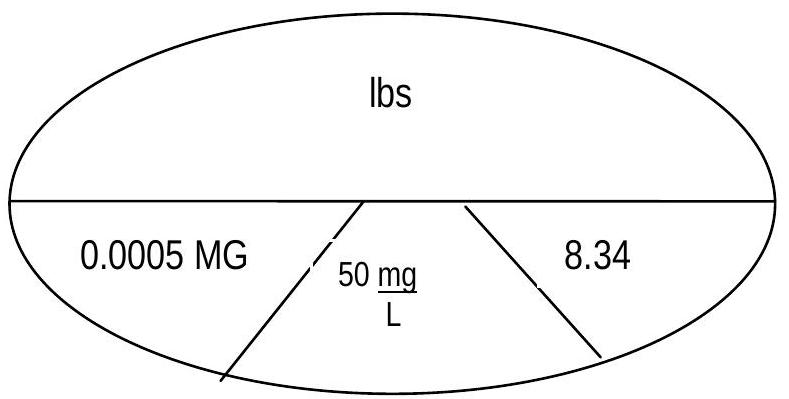
\includegraphics[max width=\textwidth]{2022_10_30_098bb5f44c5986ff92a9g-70}

Last step: Since only $65 \%$ of the calcium hypochlorite is chlorine, we need to calculate how many pounds of hypo are required to get $0.2$ pounds of chlorine. To do this we need to change the percent to a decimal and then divide the pounds required by the purity of the solution (as a decimal).
$$
\frac{0.2}{0.65}=0.3 \text { pounds }
$$

\section{Example 4.4 - Dosage Calculation}
A system has repaired the storage facility. They need to disinfect it before putting it back in service. They are going to use $25 \mathrm{mg} / \mathrm{l}$ of chlorine. How many pounds of $65 \%$ calcium hypochlorite are required if the storage facility has a 50 foot diameter and is 75 feet tall?

\section{Regulatory Monitoring and Sampling Requirements}
\section{Total Coliform Rule (TCR)}
The TCR requires all public water systems to sample for total coliform bacteria. Samples are taken at customer taps or sample taps that are representative of the distribution system. The number of required samples is dependent upon population and as specified in the system's sample siting plan.

\section{Surface Water Treatment Rule (SWTR)}
The SWTR requires public water systems using surface water sources to sample for disinfectant residual levels at the same frequency, time and locations as total coliform sampling. Depending upon disinfectant analysis results, systems may also conduct heterotrophic plate count (HPC) sampling to demonstrate compliance with the disinfectant residual performance level.

\section{Disinfection/Disinfection By-products Rule (DBPR)}
This rule requires that all public water systems that add a disinfectant to their water, meet maximum levels for Total Trihalomethane (TTHM), the sum of five haloacetic acids (HAA5), and residual disinfectant levels. The rule requires systems to collect and analyze samples from the distribution system for TTHMs and the HAA5s on a quarterly, annual, or triennial basis, depending on system type, size and previous analytical results and in accordance with the system's sampling plan. At least $25 \%$ of the TTHM samples must be collected from locations of maximum residence time. Systems must sample for residual disinfectant levels daily, monthly, or quarterly, depending upon disinfectant used, and previous analytical results. Disinfectant level samples taken to meet the SWTR requirements may also be used to meet the DBPR requirements.

\section{Lead and Copper Rule}
This rule requires community and nontransient noncommunity water systems to collect first draw samples at cold water taps in homes/buildings that are at high risk of lead or copper contamination. The number of samples sites is based on system size. Systems must conduct monitoring every six months unless they qualify for reduced monitoring to annually or triennially. Very small systems may also qualify for lead or copper nine-year monitoring waivers if they meet waiver criteria.

\section{Operations Monitoring}
\section{Water Age}
Monitoring can be used to determine if water age is negatively affecting water quality in a distribution system.

Data that can be used to analyze water age may include:

\begin{itemize}
  \item Flowrate,

  \item Velocity,

  \item Pressure,

  \item Tank levels,

  \item $\mathrm{pH}$,

  \item Disinfectant residual,

\end{itemize}
-Iron,

\begin{itemize}
  \item Color and taste,

  \item DBPs, and

  \item Heterotrophic bacteria count.

\end{itemize}
\section{Storage}
Inadequate turnover in storage facilities can have a significant negative impact on water quality within a distribution system. Monitoring at the inlets, outlets, and within storage facilities can help identify potential water quality problems and corresponding needs for modification of system operations to increase turnover.

Parameters to be monitored may include:

\begin{itemize}
  \item Total and free chlorine residual,

  \item $\mathrm{pH}$,

  \item Water temperature,

  \item Turbidity,

  \item Heterotrophic bacteria,

  \item Total coliform bacteria,

  \item Ammonia

  \item Nitrite,

  \item Taste and odor, and

  \item TTHMs.

\end{itemize}
\section{Pressure}
Monitoring of pressure at key points in the distribution system can be used to identify and resolve low or negative pressures that may lead to contamination by backflow.

Pressure monitoring should be conducted at pump stations, control valves, and high elevation points and other areas subject to low pressure.

\section{Other Purposes}
For systems that use more than one source of supply, water quality monitoring may be used to distinguish the origin of water in a distribution system.

Monitoring of disinfectant residual, heterotrophic bacteria and nitrification can be used to determine the effectiveness of booster chlorination in a distribution system.

Monitoring can be used to identify areas that may be negatively affected by an emergency event, such as a main break, repairs, or deliberate acts of terrorism.

\section{Other Monitoring}
\section{Customer Monitoring}
Customer complaints can be used to identify and resolve water quality problems. Databases of customer water quality complaints can be used to help prioritize main repair and replacement, prioritize main flushing, and determine causes of water quality problems.

\section{Secondary Standards}
Monitoring programs, which include monitoring beyond that required by regulation, may help characterize the distribution system and determine the cause of water quality problems.

\section{Distribution Flushing}
\section{Benefits}
A regular distribution flushing program can help reduce the need for reactive maintenance in a distribution system by removing biofilm and other bacteriological growth, sediment, and corrosion products and helping to prevent tuberculation.

\section{Flushing Programs}
\section{Procedures}
\begin{itemize}
  \item A flushing program involves advanced planning to outline procedures, such as the order of hydrants to be operated and valves to be closed.

  \item The flushing program should be documented.

  \item Additionally, data that may be collected during hydrant flushing, which is useful for daily system operation, includes:

  \item Repair and replacement needs,

  \item Water quality sample results, and

  \item Flow and pressure readings.

\end{itemize}
There are numerous reasons for flushing water from fire hydrants.

\begin{itemize}
  \item Testing the fire hydrants to ensure they are working properly.

  \item System flushing to expel the sediment or minerals that settles to the bottom of our water mains and help in maintaining a clean and aesthetically pleasing water supply to customers.

  \item Respond to customer complaints (one way to treat taste and odor issues).

  \item Increase chlorine residual in area of system.

  \item Expel air from new or recently repaired water lines.

\end{itemize}
Types of flushing strategies include:

\begin{itemize}
  \item Spot flushing (reactive): may be used when there are localized water quality complaints and in the case of emergencies.

  \item Routine flushing in stagnant area (short term preventative): used in problematic areas with dead ends or low demand areas to fix long detention times which can degrade water quality (a fully looped system may eliminate the need for stagnant flushing).

  \item Scheduled system-wide flushing (long term preventative): this is the most comprehensive type of flushing program which helps maintain water quality and the useful life of the mains. This is typically conducted bi-annually in the spring and fall.

\end{itemize}
Flushing methods:

\begin{itemize}
  \item Directional flushing is the recommended method of annual or semi-annual flushing to maintain water quality in the distribution system. - Requires the operator to isolate sections of water mains to allow for flushing that particular main from beginning (nearest the water plant/fresh water) to the end (furthest point).

  \item Conventional/traditional flushing is typically used in response to water quality complaints. Water moves in all direction in conventional flushing, may have low flow velocities which do not allow for system scouring.

  \item Continuous blow off is used to bled water from stagnant areas in a system. This type of flushing uses large quantities of water at flow velocities less than 1 foot per second. This type of flushing does not clean the system.

\end{itemize}
To properly clean the distribution system, it is important to keep flushing flow velocities between 5 feet per second to 12 feet per second (lower velocities for discolored water and higher velocities for sediment removal).

Fire hydrant flushing steps:

\begin{enumerate}
  \item Notify customers in particular:
\end{enumerate}
\begin{itemize}
  \item Hospitals

  \item Dialysis clinics

  \item Food processing

  \item Bottling

  \item Specialized manufacturing

\end{itemize}
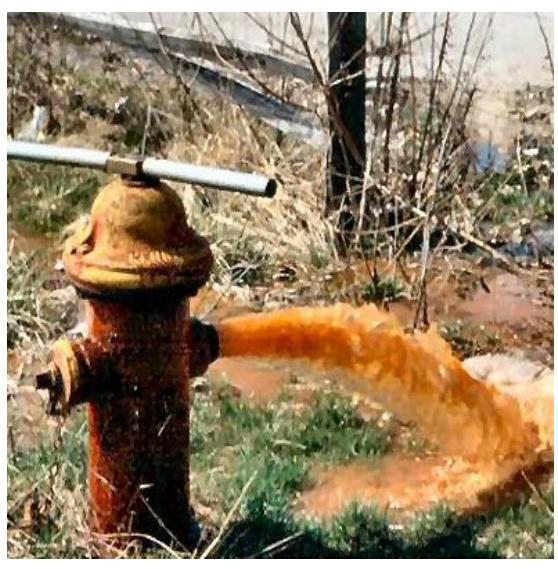
\includegraphics[max width=\textwidth]{2022_10_30_098bb5f44c5986ff92a9g-76}

\begin{enumerate}
  \setcounter{enumi}{2}
  \item Isolate section to be flushed from the rest of the system:
\end{enumerate}
\begin{itemize}
  \item Close valves slowly to prevent water hammer.
\end{itemize}
\begin{enumerate}
  \setcounter{enumi}{3}
  \item Open hydrant/blowoff valves slowly until the desired flow is obtained.
\end{enumerate}
\begin{itemize}
  \item Direct water away from traffic, pedestrians, underground utility vaults and private lands.

  \item Confirm storm drains or natural water courses can handle the flow

  \item Prevent contaminated water from discharging into sensitive areas

  \item Dechlorination may be necessary

  \item Flushing water into a tank truck may be required

\end{itemize}
\begin{enumerate}
  \setcounter{enumi}{4}
  \item Maintains $20 \mathrm{psi}$ minimum area flushing area.

  \item Record data (not including hydrant data). Page 4-17 demonstrates and example hydrant maintenance log.

  \item When water clears, close hydrant/blowoff valve slowly.

  \item Reopen valves connecting flushed section to the larger system.

  \item Proceed to next section to be flushed.

\end{enumerate}
\section{Hydrant Maintenance Log}
Date:

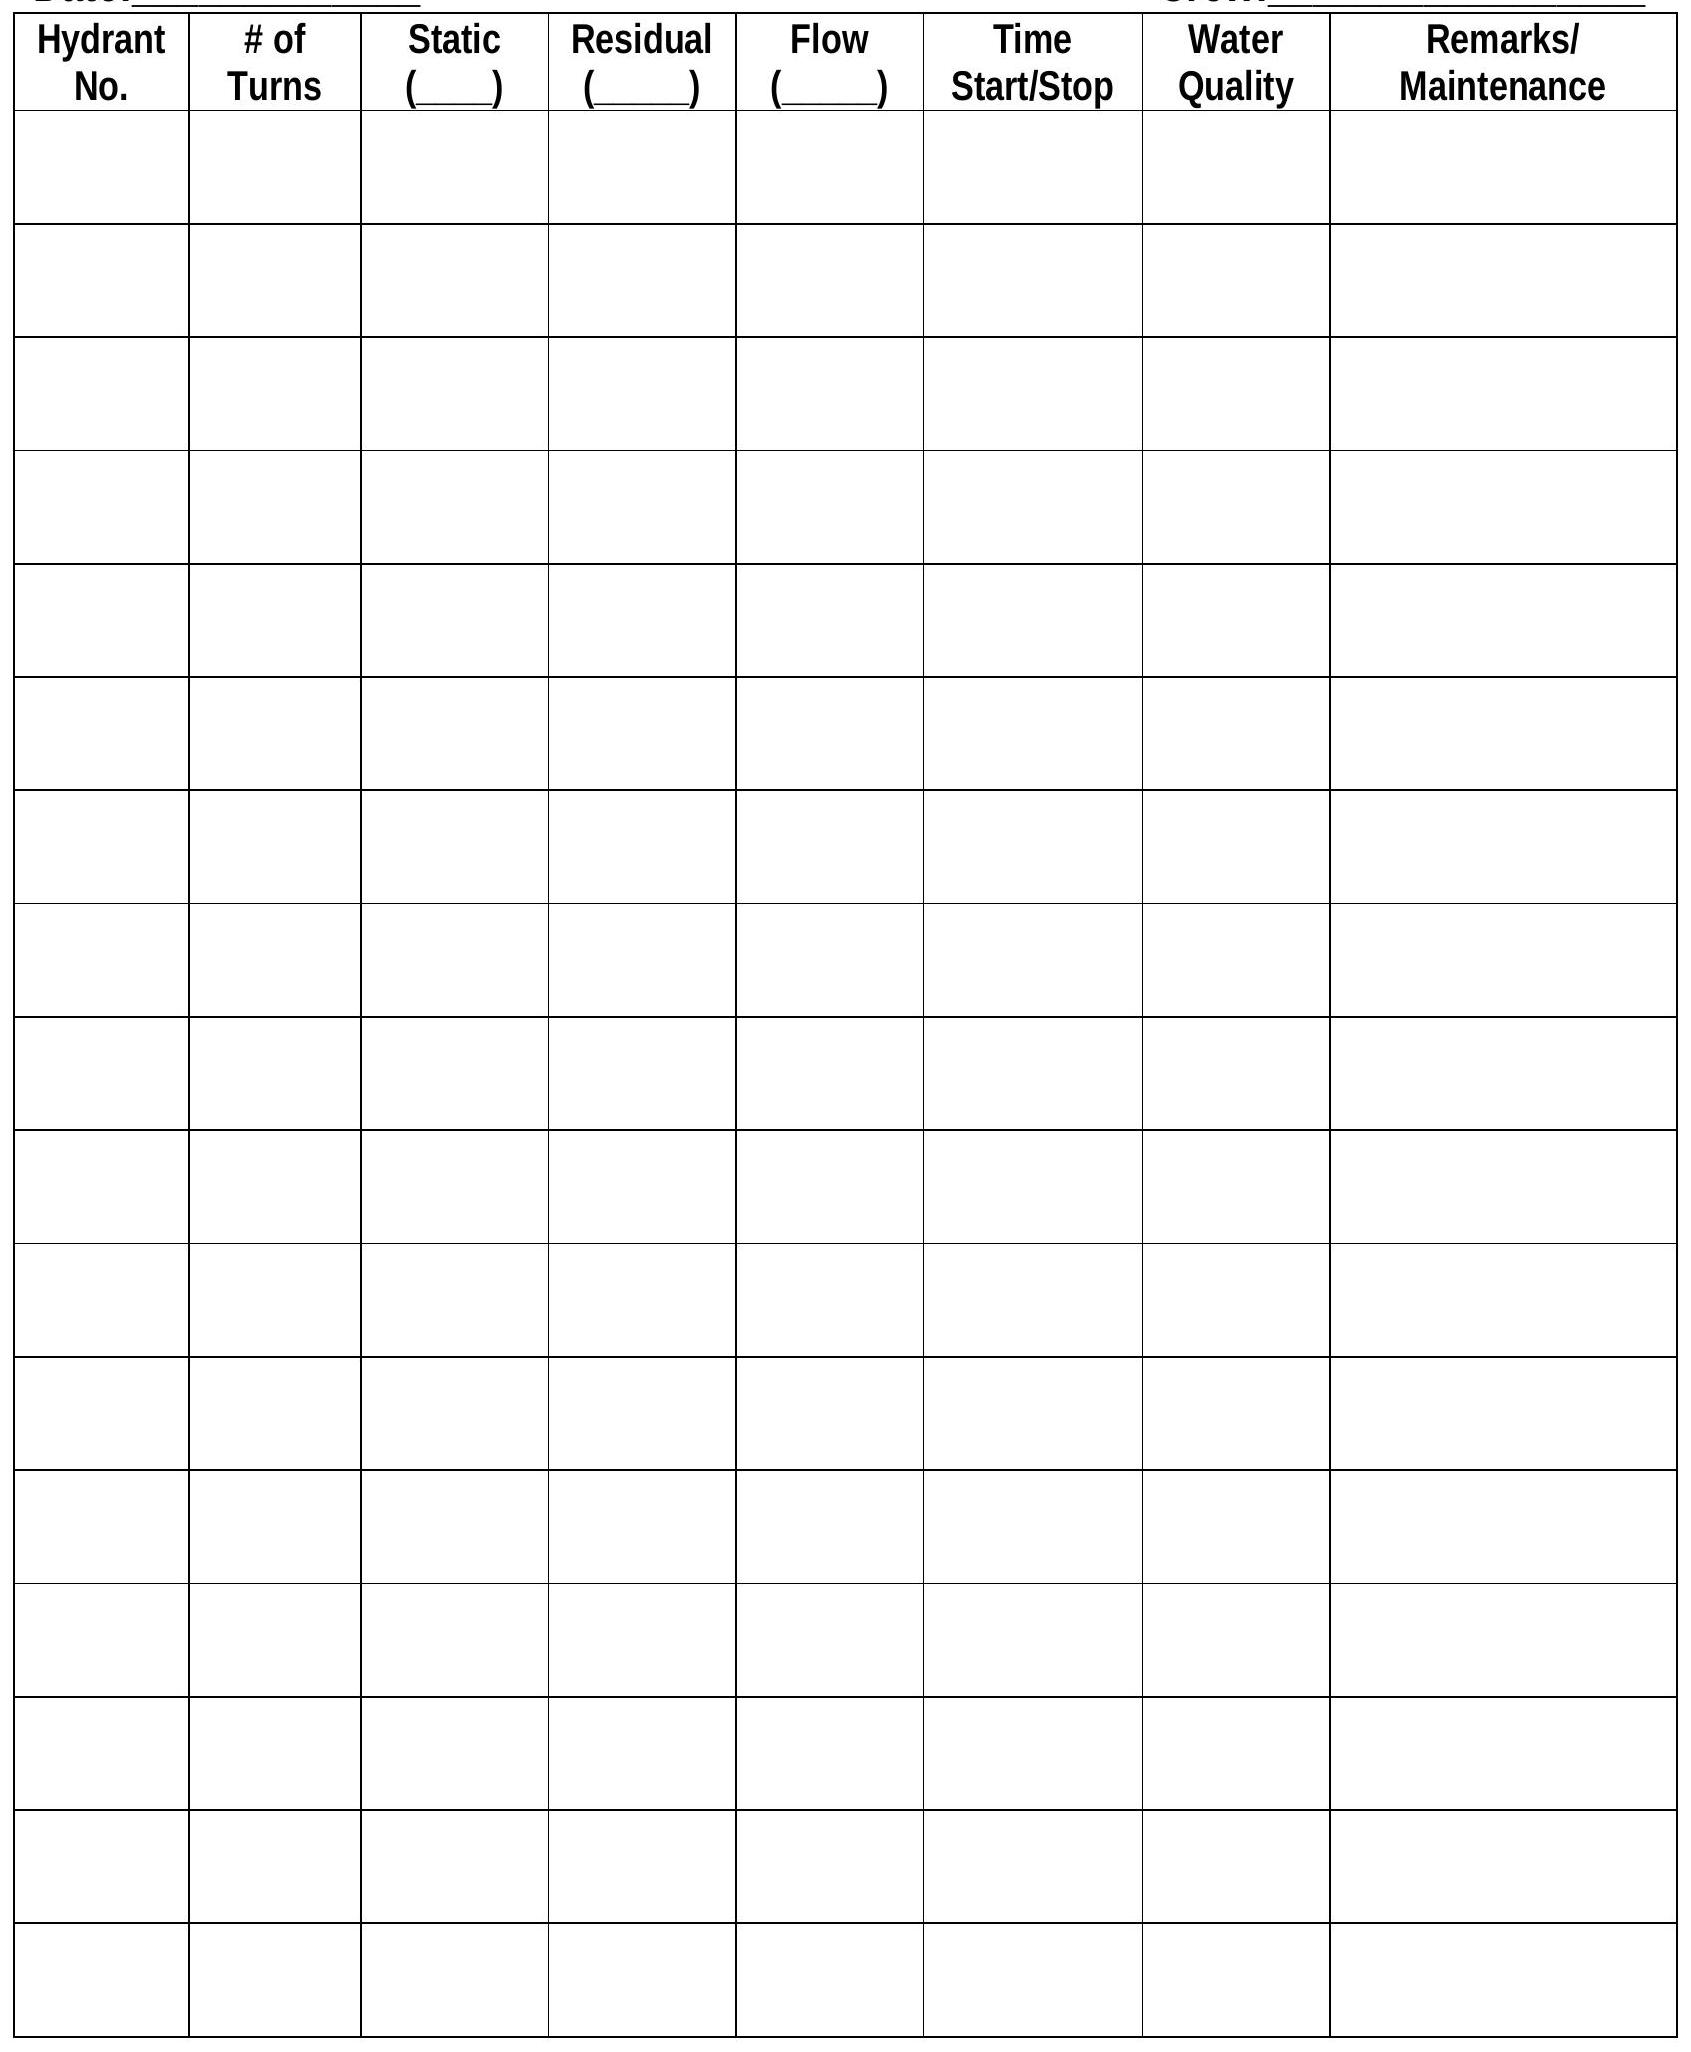
\includegraphics[max width=\textwidth]{2022_10_30_098bb5f44c5986ff92a9g-77}

\section{Cross Connection Control}
\section{Purpose}
A cross-connection is any point in a water distribution system where chemical, biological, or radiological contaminants may come into contact with potable water. During a backflow event, these contaminants can be drawn or pushed back into the potable water system. A backflow prevention device installed at every point of cross connection prevents contaminated water from entering the potable water distribution system.

\section{Primary Elements of Program}
Five key elements of an effective comprehensive cross-connection control program are as follows:

$\square$ Establish proper authority to initiate and enforce plan.

Utilize approved backflow prevention devices, test and maintain as needed.

Use only certified personnel to test devices and inspect sites.

Maintain accurate installation, testing, and inspection records.

Educate the public about the danger of cross-connection.

\section{Water Main Cleaning and Lining}
\section{Benefits}
Cleaning and lining of mains that have significant accumulation of sediment, tuberculation, and/or corrosion can be conducted to:

\begin{itemize}
  \item Improve pipeline hydraulic capacity,
\end{itemize}
$\square$ Resolve water quality problems, and

$\square$ Prevent future water quality problems.

\section{Methods of Cleaning}
Flushing

Mechanical Cleaning Methods include use of:

\begin{itemize}
  \item Pigs,

  \item Swabs,

  \item Scrapers or brushes, and

  \item Induction of air.

\end{itemize}
\section{Lining}
$\square \quad$ Lining may be desirable when the existing main is structurally sound and of sufficient diameter.

It involves applying a cement mortar lining or an epoxy to an existing pipe in order to improve flow characteristics and prevent future corrosion.

\section{Minimization of Dead Ends and Residence Times}
\section{Stagnation Issues}
Stagnation in pipelines is a primary cause of deteriorating water quality within a distribution system due to water age. Stagnation contributes to depletion of disinfectant residual, bacteriological issues, turbidity, color, taste, and odor problems. Frequently, there is a build-up of iron and manganese sediment in deadend sections as well.

\section{Potential Causes of Stagnation}
Dead-end or non-looped mains often contribute to stagnation problems. Oversized mains or extremely long stretches of main with minimal customer demands can also cause stagnation.

\section{Benefits of Looping}
Looping of dead-end mains allows for continuous flow of water through the main, thereby reducing residence times and corresponding stagnation problems.

$\square$ Looping will also help increase hydraulic capacity and improve system reliability.

\includegraphics[max width=\textwidth]{2022_10_30_098bb5f44c5986ff92a9g-80}

Figure 4.2 Looped Distribution System

\section{Storage Facility Operations}
Excessive detention time in a storage facility negatively impacts distribution system water quality. System operations, including pump controls, could be modified to reduce detention times. Design modifications to storage facility inlet/outlet piping could also be used to minimize detention times.

\section{Key Points for Unit 4 - Water Quality and Monitoring}
\begin{itemize}
  \item Distribution system water quality issues include chemical, biological, and aesthetic.

  \item Chlorine residual is a common method used to make sure that subscribers at the far ends of the distribution system are protected from biological pathogens in the drinking water.

  \item The Total Coliform Rule is a regulation that requires all public water systems to sample for total coliform bacteria.

  \item Various aspects of water in the distribution system can be monitored to help assure that the quality of water is being maintained. Examples are flowrate, disinfectant residual, color and taste, etc...

\end{itemize}
\section{Unit 4 Exercise}
\begin{enumerate}
  \item Write the two immediate steps required after a bacteria test is positive for total coliform:\\
a.\\
b.\\
a. Protect public health.\\
b. Prevent corrosion.\\
c. Reduce public confidence.\\
d. Increase taste and odor.

  \item Select the best response to complete the following true statement. Chlorine is added to a water system and is maintained throughout the distribution system to:

  \item The initial chlorine demand of the impurities in a source of water is $1.5 \mathrm{mg} / \mathrm{l}$. What is the chlorine dosage required to produce a chlorine residual of $2.0 \mathrm{mg} / /$ ?

  \item What is the recommended minimum water velocity when flushing water distribution piping?

  \item List five problems associated with stagnation of water due to dead ends:\\
a.\\
b.\\
C.\\
d.\\
e. 6. A system has replaced 350 feet of 12 inch water main. They are going to use $50 \mathrm{mg} / \mathrm{l}$ of chlorine for 24 hours to disinfect the line. How many pounds of $65 \%$ calcium hypochlorite are required? 1.Report of Daniel D. Jackson, Sanitary and Chemical Engineer, Executive Officer of the Dept. of Chemical Engineering of Columbia University, November, 1928.

\end{enumerate}
2 "Community Water Systems," Public Water Supply Manual, (PA DEP) Part II p. 7.0.18.

\section{Additional Resources Used}
"Community Water Systems," Public Water Supply Manual, (PA DEP) Part II p. 7.0.18, Part IV 1.1.

"Distribution Components and Disinfection Student Manual," (PA Rural Water Association, Bellefonte, PA: PRWA) p. 21-29.

"Guidance for Management of Distribution System Operation and Maintenance," American Water Works Association Research Foundation \#2, (AWWA Research Foundation, Denver, CO: AWWARF) p.30$34,32-40,41-43,61-67,75-77,89-93,99$.

"Guidance Manual for Monitoring Distribution System Water Quality," American Water Works Association Research Foundation \#4, (AWWA Research Foundation, Denver, CO: AWWARF) p. 65-70, $75,77-82,96-97$.

"Guidance Manual for Monitoring Distribution System Water Quality," AWWA Water Distribution System Operation and Maintenance, (AWWA Denver, CO: University of California at Sacramento) p.2.42, $5.706,5.707,5.708$.


\end{document}